%%%% ijcai17.tex

\typeout{}

% These are the instructions for authors for IJCAI-17.
% They are the same as the ones for IJCAI-11 with superficical wording
%   changes only.

\documentclass{article}
% The file ijcai17.sty is the style file for IJCAI-17 (same as ijcai07.sty).
\usepackage{ijcai17}
\usepackage{CJK}

% Use the postscript times font!
\usepackage{times}

\usepackage{amsmath,amsfonts}
\usepackage{color}
\usepackage{url}
\usepackage{array}
\usepackage{epsfig}
\usepackage{graphicx}
\usepackage{subcaption}

% the following package is optional:
%\usepackage{latexsym} 

% Following comment is from ijcai97-submit.tex:
% The preparation of these files was supported by Schlumberger Palo Alto
% Research, AT\&T Bell Laboratories, and Morgan Kaufmann Publishers.
% Shirley Jowell, of Morgan Kaufmann Publishers, and Peter F.
% Patel-Schneider, of AT\&T Bell Laboratories collaborated on their
% preparation.

% These instructions can be modified and used in other conferences as long
% as credit to the authors and supporting agencies is retained, this notice
% is not changed, and further modification or reuse is not restricted.
% Neither Shirley Jowell nor Peter F. Patel-Schneider can be listed as
% contacts for providing assistance without their prior permission.

% To use for other conferences, change references to files and the
% conference appropriate and use other authors, contacts, publishers, and
% organizations.
% Also change the deadline and address for returning papers and the length and
% page charge instructions.
% Put where the files are available in the appropriate places.

\newcommand{\secref}[1]{Section \ref{#1}}
\newcommand{\figref}[1]{Figure \ref{#1}}
\newcommand{\eqnref}[1]{Eq. (\ref{#1})}
\newcommand{\tabref}[1]{Table \ref{#1}}
\newcommand{\exref}[1]{Example \ref{#1}}
\newcommand{\argmin}{\operatornamewithlimits{argmin}}
\newcommand{\argmax}{\operatornamewithlimits{argmax}}
\newtheorem{example}{Example}
\newtheorem{lemma}{Lemma}
\newtheorem{definition}{Definition}
\newcommand{\cut}[1]{}

\newcommand{\li}{\uline{\hspace{0.5em}}}
\newcommand{\BL}[1]{\textcolor{blue}{Bill: #1}}
\newcommand{\HY}[1]{\textcolor{red}{Hanyuan: #1}}
\newcommand{\KZ}[1]{\textcolor{green}{Kenny: #1}}
\newcommand{\SH}[1]{\textcolor{green}{Seung: #1}}
\newcommand{\FX}[1]{\textcolor{blue}{Frank: #1}}


\title{Representing Cross-cultural Bilingual Terms by Socio-linguistic Features}
\author{}

\begin{document}
\begin{CJK}{UTF8}{gbsn}

\maketitle

\begin{abstract} 
Capturing cultural differences is an important challenge in bilingual text understanding
or machine translation. This paper presents a novel framework for obtaining cross-lingual 
term representations by mining sociolinguistic features from online social media. 
Such representations can act as a building block for computational social science tasks. 
We evaluated our framework on two such tasks: detection of cultural differences in named entities
and extraction of bilingual lexicon for online slangs. Results shows that the proposed 
socio-linguistic representation outperforms a number of baseline methods by substantial
margins.
\end{abstract}

%\IEEEraisesectionheading{
% %\IEEEraisesectionheading{
% %\IEEEraisesectionheading{
% \input{intro}
\section{Introduction}\label{sec:intro}
 %}
% \section{Introduction}\label{sec:intro}

% \begin{enumerate}
% \item Motivation: application scenarios (with 1-2 running examples);
% \item Characteristics of the data sources and their challenges;
% \item Briefly introduce previous approaches to extract information 
% from images including setting the document zone, and their limitations.
% \item General flow of our approach (may give a diagram here)
% \end{enumerate}
% scenary

Due to ever evolving hardware and software, many medical images
such as electro-cardio graphs (ECGs), X-ray or ultrasound images  
are directly printed and stored in hard copy formats. 
% \KZ{Insert 4 example images here.}
%Examples are shown in \figref{fig:medicalImages}. 
% These images often contain a mix of graphics and text, which
% include parameter settings of the hardware, test measurements or simple
% diagnosis. 
These images often contain a mix of graphics and text, which 
include technical settings of the hardware used, test measurements or simple diagnoses.
Recently, there has been a growing demand for digitizing such 
medical information from paper media sources, especially legacy ones, or patients who want to keep track of these documents by themselves digitally. 
Apart from scanning the graphics into a digital format, extracting 
the semi-structured textual information is also an important part of
building electronic medical records for patients. 

%\begin{figure}[!htb]
%\centering
%\subfloat[ECG]{
%\label{fig:medicalimage:ecg}
%\epsfig{file=figure/17_ori.eps, width=0.4\columnwidth}
%}
%% \hfill
%\subfloat[MRI]{
%	\label{fig:medicalimage:mrt}
%	\epsfig{file=figure/MRI.eps, width=0.4\columnwidth}
%}
%\\
%\subfloat[X-RAY]{
%\label{fig:medicalimage:xray}
%\epsfig{file=figure/X-RAY.eps, width=0.4\columnwidth}
%}
%%\hfill
%\subfloat[EEG]{
%\label{fig:medicalimage:eeg}
%\epsfig{file=figure/EEG.eps, width=0.4\columnwidth}
%}
%\caption{Examples of Medical Images}
%\label{fig:medicalImages}
%\end{figure}

Optical character recognition (OCR)  \cite{mori1992historical,smith2007overview} is 
a traditional technique used to turn images of printed text into machine encoded
text. It is well researched and performs well on plain text 
documents such as novels and reports, for a variety of languages. 
%For example, Tesseract, which is one of 
%the most popular open source multilingual recognizers, logs an error 
%rate of 3.72\% for English words and 3.77\% for simplified 
%Chinese characters\cite{smith2009adapting}. 
%Google Books \cite{googlebooks} and Gutenberg \cite{gutenberg} are
%projects which have scanned a large number of paper books into text for free and open
%access. These projects made exclusive use of OCR for this conversion and 
%achieved high accuracy \cite{vincent2007google} \cite{lebert2008project}. 
% 99\% for Gutenberg project \cite{lebert2008project}. 
% \KZ{Give the accuracy of google and gutenberg if available.}


\begin{figure}[th]
\centering
\epsfig{file=figure/17_b.eps, width=0.8\columnwidth}
\caption{An ECG image with text area (red circle) of interest.}
\label{fig:ecgexample2}
\end{figure}

For a semi-structured medical image, such as 
\figref{fig:ecgexample2}, we would like to extract the attribute-value 
pairs (e.g., {\em Vent. rate = 63 bpm}) and possibly other values such as
date ({\em 18-Nov-2010}) and time ({\em 9:13:02}) since those values endow us with lots of information about the patient. 
Existing OCR software cannot extract such structured information in a straightforward 
fashion, 
but instead it produces rather convoluted results from the whole image, 
similar to those in \figref{fig:ocrre}, which was produced by Tesseract, 
a popular multi-lingual recognizers. 
% \KZ{Maybe include the x-y coordinate info in the output as well?}  

\begin{figure}[th]
\centering
\scriptsize
\begin{verbatim}
<p class="ocr_par" title="box 263 33 444 119">
   <span class="ocr_l" title="box 264 33 336 45">
       <span class="ocrx_w" title="box 264 33 299 45">Vcnt.</span> 
       <span class="ocrx_w" title="box 308 34 336 45">rule</span> 
   </span>
   <span class='ocr_l'>
       <span class="ocrx_w" title="box 264 51 283 64">PR</span> 
       <span class="ocrx_w" title="box 291 51 346 64">Interval</span> 
       <span class="ocrx_w" title="box 389 52 411 64">140</span> 
       <span class="ocrx_w" title="box 420 55 439 64">ms</span> 
   </span>
   ...
   </span>
</p>
<p class="ocr_p" dir="ltr">
   <span class="ocr_l">
       <span class="ocrx_w" title="box 396 33 411 45">53</span> 
       <span class="ocrx_w" title="box 420 33 449 48">bpm</span> 
   </span>
</p>
\end{verbatim}
\caption{Snippet OCR results in XML, input to our framework.}
\label{fig:ocrre}
\end{figure}


%\input{xmlre1}

%However, OCR alone does not work well on semi-structured text and hence
%can't be directly used for information extraction from the aforementioned
%medical images. \KZ{Give the reason here, perhaps because OCR models are
%largely Markov based? So semi-structured data breaks the flow of text.}
%When a medical image is input to an ordinary OCR software, the spatial 
%information of the text components is often lost or mixed with noises
%and errors.
%%The reason is OCR converts the whole images into text data, in which 
%%useful information often mix with noises and errors. 
%In this paper, we would like to extract the attribute-value pairs
%and possibly other values from \figref{fig:ecgexample1} 
%and \figref{fig:ecgexample2}. 
%% or medical ultrasonography report. 
%Such images contain lots of non-textual information or noises.

% example & ref
%\begin{figure}[ht]
%\centering
%\epsfig{file=figure/46.eps, width=0.8\columnwidth}
%\caption{ECG Images From Printer1}
%\label{fig:ecgexample1}
%\end{figure}

% \begin{figure}[ht]
% \centering
% \subfloat[Printer1]{
% \label{fig:ecgexample:a}
% \epsfig{file=figure/46.eps, width=0.48\columnwidth}
% }
% \hfill
% \subfloat[Printer2]{
% \label{fig:ecgexample:b}
% \epsfig{file=figure/17.eps, width=0.48\columnwidth}
% }
% \caption{ECG images from two different printers}
% \label{fig:ecgexample}
% \end{figure}

Also, errors in the OCR text \cite{darwish2007error,taghva1996evaluation} will greatly affect the effectiveness 
of other related tasks. Much work has been done to improve the performance of the OCR\cite{kolak2003generative,cesarini1998informys}. However, there are still a number of significant challenges involved in extracting the information from medical images or OCR results in XML form. 

% First, medical images differ from pure text document in that them have 
% layout information. 
First, medical images differ from pure text documents in that 
they contain layout information.
Although most current OCR engines attempt to reproduce the physical 
layout of the text units, 
%(along with X-Y coordinates) and store them 
%in a special format such as XML 
% (\KZ{Better in the previous example})
such spatial
information is approximate and sometimes inaccurate, which is why neighboring
text blocks in \figref{fig:ecgexample2}, such as ``Vent. Rate'' and
``63 bpm'' were not automatically combined into the same XML block, but were 
rather far apart (shown in two different ``classes'') in \figref{fig:ocrre} made by OCR softwares. 
%Even for images produced by the same ECG printer, 
%the XML results can still be very different as 
The spatial layout is sensitive to many factors, such as accidental spots 
on the prints, color and contrast, or the angle of the camera. 
%In this case, solutions for other application domains, for example, the web, 
%are not well suited for information extraction from printed documents \cite{bartoli2014semisupervised}. With such inaccurate
%layout information produced by OCR,
%it is not easy to write a simple wrapper program to extract useful
%data from images, even if the images come from the same printer. 

%Writing a wrapper for each
%individual image would be tedious and counter-productive. Therefore,
%a mechanism that makes use of the spatial locality of the 
%text units in the image and 
%accommodates slight variations in the spatial layout would make the extraction
%more accurate and fault-tolerant.

%For example, \figref{fig:ocrre} is the simplified OCR results for the ECGs in 
%\figref{fig:ecgexample1} and \figref{fig:ecgexample2}. The results are in the XML format and have attritube named {\em class} 
%for layout information. Although these two images share similar format. 
%OCR engine generates different results in that it splits elements that 
%should be in the same line into two lines in the second example. 
%XML is sensitive to the layout results so it's hard to tolerate 
%all the layout results. 
%
% example check the term
% layout of ocr results can be restore, so why OCR engine don't restore the results 
% using the similar methods as we do?
% or the way we handle the layout problem is quite simple

% Delete for TIP
% Second, exiting OCR engines make heavy use of Markov properties such as n-grams
% since they primarily target the transformation of large body of text 
% \cite{kolak2003generative}. 
% % \KZ{Needs some refs here.}
% Unfortunately, the semi-structured texts in medical images are often 
% short and not even written in complete sentences, thus breaking Markov assumption. To make
% matters worse, medical images contain scientific language, which may be
% very different from the training corpora of these OCR engines.
% This explains why we see errors like ``Vcnt'' and ``rule'' 
% in \figref{fig:ocrre}. 
% %can't guarantee a perfect performance, which means 
% %there are errors and noises in the OCR results.
% %Many of them due to the fact that the data are no longer long, continous
% %sentences, thus breaking the Markov assumption made by many OCR algorithms. 
% %In \figref{fig:ocrresub:b}, ``Vent." is misrecognized as ``Vcnt.". 
% Without sufficient contextual information, OCR may also misrecognize a 
% digit as an alphabetic character, or as another similar digit. 
% Furthermore, the mix of text with images and formatting
% lines often confuses the OCR engine, which is more biased toward full
% text images.
% Exact pattern matching, as used in
% traditional information extraction, doesn't work with such noisy OCR output
% as it doesn't tolerate noises or errors in text. 
% %It's hard to autocorrect these errors 
% %because image quality is the most important affecting factor. 
% %The text we are processing can be full of no meaning words or 
% %strange numbers. 
% A fuzzy matching strategy is more desirable in this case. 
% % example, what are the traditional IEs

Second, there are many types of medical images, resulting from a variety of
medical tests. Different equipments for the same test can produce vastly 
different images. Writing individual extraction wrappers 
for the OCR outputs of all these formats is tedious and inefficient, 
and difficult for non-programmers.
%not to mention that there are significant programming barriers for 
%writing these wrappers, especially for the medical professionals who are the
%end users of these extraction results. 
%A more user-friendly approach enabling users to specify such extraction requirements would be preferred. 
%There are various kinds of medical images, such as electrocardiograph report, 
%medical ultrasonography report, etc. 
%However the basic measures for each type of medical test (e.g., ECG), 
%are very similar from machine to machine. Only the layouts are 
%different. 
% example medical images

Finally, most off-the-shelf OCR programs are pre-trained with specific 
recognition models, which may not be suitable for the extraction of 
%medical images.
%Furthermore, changes in imaging equipment technology over time may produce 
%different formats, layout, or terminology, rendering existing OCR models 
%obsolete. 
Re-training the models requires a large amount of labeled data, which may
not be available. 
%Incremental training as more labeled data arrives
%is currently not supported by any OCR product.    

%There have been some limited attempts to address some of the above challenges. 
%One solution is a plugin of an OCR program that allows the user to specify 
%target zones of interest in the image to be extracted. The zones specified for
%one image can be applied to images with slight variations by adjusting against
%a fixed reference point that is supposed to exist in all these images.
%% \KZ{I think the problem is not so much with the zones, because we also
%% have zones, but rather with the reference point.}
%% \JY{}
%% example products
%% http://www.square-9.com/automated-data-extraction-optical-character-recognition
%The problem with this solution is its high reliance on the OCR zones  
%established by the user. The performance of the results is affected by the 
%accuracy of the zones. If the zones are too big, the results will be full of 
%noise. If the zones are too small, results will miss something. 
%
%Another solution involves using the page layout analysis technique. The page layout 
%analysis technique is used to determine where the text 
%resides on a page \cite{o1993document}, 
%% \KZ{This page layout analysis approach is not clearly described. I don't understand after reading this paragraph.}
%% By using page layout analysis technique, the hierarchy of physical components 
%% can be generated and to match with the hierarchy of logical components, which 
%% is predefined. 
%this includes identifying and categorizing the 
%regions of interest in the scanned image of a text document. 
%Typically, the first step is to segment text zones from 
%non-textual zones and arrange them in their original order. 
%Then in order to analyze the logical roles of the text zones 
%(titles, captions, footnotes, etc.), logical layout analysis 
%is used for labeling the semantics of the text zones.
%Generally, page layout analysis is used for documents. The problem with applying 
%such a technique on medical images is that it creates so much noises 
%that performance is ultimately affected. 
%For medical imaging reports like ECG, useful information is often 
%found in the small components of the image, while most of the images are 
%read as noises. 
% check paper and more description, weakness, ref

%In this paper, 
%we propose a spatial data description language, which borrows its syntax from
%PADS \cite{fisher+:pads}, an ad hoc data processing language, 
%for describing semi-structured data in medical images. 
%% ref
%We call this language OCR description language, or ODL. 
%ODL is designed for extracting and parsing semi-structured text data 
%from images. We believe that  information extraction from those data in ODL form may be much easier than extracting information from rough data or data in XML form, which means that our preprocessing part proves to be necessary.
%%An example ODL description for the image in 
%%\figref{fig:ecgexample2} is shown in 
%%\figref{fig:description}. \KZ{Make this description two column, and give
%%some brief explanation of this description here.} 
%%The parsing result of this description is shown
%%in \figref{fig:parsing result}. \KZ{Give some explanation of the results,
%%otherwise don't show the result here. E.g., you need to explain what F, E, etc.
%%mean. You want to say that even though rate has been recognized as rule,
%%the bpm value was still extracted (but still wrong!).}
%% \KZ{I removed the preprocessing part, cos it's not important. Talk about it in
%% discussion sec.}
%%The our approach starts by preprocessing the images for text results.
%To use this framework, the user first describes the components in the image
%that he or she is interested in extracting. This includes constant strings
%and variables of different data types.   
%ODL allows the user to specify the approximate spatial layout and constraints on
%the data, e.g., integers within 
%a certain range, real numbers with certain decimal points, etc. 
%%This information is then as the key component in our fuzzy matching strategy. 
%The system then automatically generates a parser for these medical images.
%This parser uses the output XML from OCR with spatial information as an input, 
%and outputs a data structure with values extracted for each variables
%in the description, unless there is an unrecoverable error during the parsing process.
%In addition, approximate layout information and constraints are used in parsing process 
%to tolerate noises and small format variations in the input images. 
%%Specifically, this method could be called fuzzy matching, meaning that more candidates could be saved after the parsing process.  It's obvious that we may have a higher probability to obtain the accurate result if more candidates are kept so that fuzzy match should be used properly in our system.
%%An autogenerated parser based on the ODL description can release us from 
%%repetitive work. In this way, we turn the task of writing complex parsers 
%%into describing information on images.
%
%
%When users process many images of the same format, the system 
%automatically discovers parsing errors given the current model and 
%prompts the user to manually correct some of the frequent and prominent
%errors, which effectively serves as an online labeling function. 
%These incrementally labeled data are then used to update the parsing model. 


%It should be emphasized that the incremental learning model is very important in our whole system. Incremental learning is a machine learning paradigm where the learning process takes place whenever we have new examples or data added to our baisc data set, leading to a most striking difference between incremental learning and traditional machine learning: it does not assume the availability of a sufficient training set before the learning process. What incremental learning in our system is really impressive: it does not require a relatively good and stable training set at first time. In fact, it could improve the parsing result with even relatively rough training sets at first by absorbing new data or corrective information as time passes in dynamic systems. Besides, the process would be very effective when there are some new images coming in since training process would not learn from scratch, which might waste time and computation resource.

%At last, we propose an incrementally human correction framwork which can 
%make the best use of human correction to handle the misrecognition problem. 
% Base on our experiments on about 500 real life ECG images, 
% our approach achieves p1 and p2 after p3 times human correction. 
% experimental results

% \begin{figure}[h]
% \begin{lstlisting}
% Oenum str_month_t{
% 	"Jan", "Feb", "Mar", "Apr",
% 	"May", "Jun", "Jul", "Aug",
% 	"Sept", "Oct", "Nov", "Dec"
% };

% Ounion month_t{
% 	Oint(1,12)	num;
% 	str_month_t	str;
% };

% Ostruct time_t{
% 	Oint(1,31)	day;
% 	"-";
% 	month_t	month;
% 	"-";
% 	Oint	year;
% };

% Ostruct triple_t{
% 	"Vent.";
% 	hskip(\s)	skip1;
% 	"rate";
% 	Oint x;
% 	"bpm";
% 	vskip(\n)	skip2;
% };

% Oscource Ostruct entry_t{
% 	time_t(<-,-,-,0.3l>) t;
% 	triple_t(<0.1w,-,0.5w,->) d;
% };
% \end{lstlisting}
% \caption{Description}\label{fig:description}
% \end{figure}


In order to solve above problems, We design a system which makes three main contributions:
\begin{enumerate}
\item Based on some previous work on data description language \cite{lamport1986document,taft1999post,fisher+:pads},we design a new declarative spatial data description language called \textit{OCR description language}, or ODL,
which allows users to specify spatial and data constraints in medical 
images(\secref{sec:syntax});
\item We propose a noise-tolerant parser which takes OCR results
the ODL description as input and outputs a data structure with values 
extracted for each variables in the description (\secref{sec:semantics});
\item We propose an incremental manual correction 
framework\cite{von2008recaptcha,zhu2012learnpads++}, which 
takes advantage of user corrections  and improves the productivity
significantly (\secref{sec:correction}).
%To be more specific, the framework improves the traditional machine learning methods by using a incremental learning process to avoid starting from scratch when we are trying to apply human corrections in the system. That means the framework would be more effective than most corrective systems.
\end{enumerate}


\section{Introduction}\label{sec:intro}
 %}
% \section{Introduction}\label{sec:intro}

% \begin{enumerate}
% \item Motivation: application scenarios (with 1-2 running examples);
% \item Characteristics of the data sources and their challenges;
% \item Briefly introduce previous approaches to extract information 
% from images including setting the document zone, and their limitations.
% \item General flow of our approach (may give a diagram here)
% \end{enumerate}
% scenary

Due to ever evolving hardware and software, many medical images
such as electro-cardio graphs (ECGs), X-ray or ultrasound images  
are directly printed and stored in hard copy formats. 
% \KZ{Insert 4 example images here.}
%Examples are shown in \figref{fig:medicalImages}. 
% These images often contain a mix of graphics and text, which
% include parameter settings of the hardware, test measurements or simple
% diagnosis. 
These images often contain a mix of graphics and text, which 
include technical settings of the hardware used, test measurements or simple diagnoses.
Recently, there has been a growing demand for digitizing such 
medical information from paper media sources, especially legacy ones, or patients who want to keep track of these documents by themselves digitally. 
Apart from scanning the graphics into a digital format, extracting 
the semi-structured textual information is also an important part of
building electronic medical records for patients. 

%\begin{figure}[!htb]
%\centering
%\subfloat[ECG]{
%\label{fig:medicalimage:ecg}
%\epsfig{file=figure/17_ori.eps, width=0.4\columnwidth}
%}
%% \hfill
%\subfloat[MRI]{
%	\label{fig:medicalimage:mrt}
%	\epsfig{file=figure/MRI.eps, width=0.4\columnwidth}
%}
%\\
%\subfloat[X-RAY]{
%\label{fig:medicalimage:xray}
%\epsfig{file=figure/X-RAY.eps, width=0.4\columnwidth}
%}
%%\hfill
%\subfloat[EEG]{
%\label{fig:medicalimage:eeg}
%\epsfig{file=figure/EEG.eps, width=0.4\columnwidth}
%}
%\caption{Examples of Medical Images}
%\label{fig:medicalImages}
%\end{figure}

Optical character recognition (OCR)  \cite{mori1992historical,smith2007overview} is 
a traditional technique used to turn images of printed text into machine encoded
text. It is well researched and performs well on plain text 
documents such as novels and reports, for a variety of languages. 
%For example, Tesseract, which is one of 
%the most popular open source multilingual recognizers, logs an error 
%rate of 3.72\% for English words and 3.77\% for simplified 
%Chinese characters\cite{smith2009adapting}. 
%Google Books \cite{googlebooks} and Gutenberg \cite{gutenberg} are
%projects which have scanned a large number of paper books into text for free and open
%access. These projects made exclusive use of OCR for this conversion and 
%achieved high accuracy \cite{vincent2007google} \cite{lebert2008project}. 
% 99\% for Gutenberg project \cite{lebert2008project}. 
% \KZ{Give the accuracy of google and gutenberg if available.}


\begin{figure}[th]
\centering
\epsfig{file=figure/17_b.eps, width=0.8\columnwidth}
\caption{An ECG image with text area (red circle) of interest.}
\label{fig:ecgexample2}
\end{figure}

For a semi-structured medical image, such as 
\figref{fig:ecgexample2}, we would like to extract the attribute-value 
pairs (e.g., {\em Vent. rate = 63 bpm}) and possibly other values such as
date ({\em 18-Nov-2010}) and time ({\em 9:13:02}) since those values endow us with lots of information about the patient. 
Existing OCR software cannot extract such structured information in a straightforward 
fashion, 
but instead it produces rather convoluted results from the whole image, 
similar to those in \figref{fig:ocrre}, which was produced by Tesseract, 
a popular multi-lingual recognizers. 
% \KZ{Maybe include the x-y coordinate info in the output as well?}  

\begin{figure}[th]
\centering
\scriptsize
\begin{verbatim}
<p class="ocr_par" title="box 263 33 444 119">
   <span class="ocr_l" title="box 264 33 336 45">
       <span class="ocrx_w" title="box 264 33 299 45">Vcnt.</span> 
       <span class="ocrx_w" title="box 308 34 336 45">rule</span> 
   </span>
   <span class='ocr_l'>
       <span class="ocrx_w" title="box 264 51 283 64">PR</span> 
       <span class="ocrx_w" title="box 291 51 346 64">Interval</span> 
       <span class="ocrx_w" title="box 389 52 411 64">140</span> 
       <span class="ocrx_w" title="box 420 55 439 64">ms</span> 
   </span>
   ...
   </span>
</p>
<p class="ocr_p" dir="ltr">
   <span class="ocr_l">
       <span class="ocrx_w" title="box 396 33 411 45">53</span> 
       <span class="ocrx_w" title="box 420 33 449 48">bpm</span> 
   </span>
</p>
\end{verbatim}
\caption{Snippet OCR results in XML, input to our framework.}
\label{fig:ocrre}
\end{figure}


%% \begin{figure}[ht]
% \centering
% \subfigure[]{
% \label{fig:subfig:a}
% \begin{minipage}[b]{0.2\textwidth}
%\newsavebox{\firstlisting}
%\begin{lrbox}{\firstlisting}% Store first listing
%\begin{lstlisting}
%<p class='ocr_par' dir='ltr'>
%   <span class='ocr_line' id='line_2'>
%       <span class='ocrx_word' id='word_6'>Vent.</span>
%       <span class='ocrx_word' id='word_7'>rate</span>
%       <span class='ocrx_word' id='word_8'>65</span>
%       <span class='ocrx_word' id='word_9'>bpm</span>
%   </span>
%   <span class='ocr_line' id='line_3'>
%       <span class='ocrx_word' id='word_14'>PR</span>
%       <span class='ocrx_word' id='word_15'>interval</span>
%       <span class='ocrx_word' id='word_16'>162</span>
%       <span class='ocrx_word' id='word_17'>ms</span>
%   </span>
%    ...
%</p>
%\end{lstlisting}
%\end{lrbox}
% \end{minipage}
% }
% \hspace[1in]
% \subfigure[]{
% % \label{fig:subfig:b}
% % \begin{minipage}[b]{0.2\textwidth}
\newsavebox{\secondlisting}
\begin{lrbox}{\secondlisting}
% \tiny
\begin{lstlisting}[basicstyle=\tiny,]
<p class="ocr_par" title="box 263 33 444 119">
   <span class="ocr_l" title="box 264 33 336 45">
       <span class="ocrx_w" title="box 264 33 299 45">Vcnt.</span>
       <span class="ocrx_w" title="box 308 34 336 45">rule</span>
   </span>
   <span class='ocr_l'>
       <span class="ocrx_w" title="box 264 51 283 64">PR</span>
       <span class="ocrx_w" title="box 291 51 346 64">Interval</span>
       <span class="ocrx_w" title="box 389 52 411 64">140</span>
       <span class="ocrx_w" title="box 420 55 439 64">ms</span>
   </span>
   ...
   </span>
</p>
<p class="ocr_p" dir="ltr">
   <span class="ocr_l">
       <span class="ocrx_w" title="box 396 33 411 45">53</span>
       <span class="ocrx_w" title="box 420 33 449 48">bpm</span>
   </span>
</p>
\end{lstlisting}
\end{lrbox}
% % \end{minipage}
% }

% \KZ{\figref{fig:ocrre} is output from what software? Tesseract?}
\begin{figure*}[th]
%\subfloat[Image From Printer1]{
%\label{fig:ocrresub:a}
%\scalebox{0.8}{\usebox{\firstlisting}}}
%\hfill
%\subfloat[Image From Printer2]{
\scalebox{1.6}{\usebox{\secondlisting}}
% \label{fig:ocrre}
\caption{A fragment of raw OCR results for ECG with layout information.}
%\caption{Simplified OCR Results in XML for an ECG with Layout Information}
%\label{fig:ocrresub:b}
\label{fig:running-xml}
\end{figure*}

% \lipsum[2]


%However, OCR alone does not work well on semi-structured text and hence
%can't be directly used for information extraction from the aforementioned
%medical images. \KZ{Give the reason here, perhaps because OCR models are
%largely Markov based? So semi-structured data breaks the flow of text.}
%When a medical image is input to an ordinary OCR software, the spatial 
%information of the text components is often lost or mixed with noises
%and errors.
%%The reason is OCR converts the whole images into text data, in which 
%%useful information often mix with noises and errors. 
%In this paper, we would like to extract the attribute-value pairs
%and possibly other values from \figref{fig:ecgexample1} 
%and \figref{fig:ecgexample2}. 
%% or medical ultrasonography report. 
%Such images contain lots of non-textual information or noises.

% example & ref
%\begin{figure}[ht]
%\centering
%\epsfig{file=figure/46.eps, width=0.8\columnwidth}
%\caption{ECG Images From Printer1}
%\label{fig:ecgexample1}
%\end{figure}

% \begin{figure}[ht]
% \centering
% \subfloat[Printer1]{
% \label{fig:ecgexample:a}
% \epsfig{file=figure/46.eps, width=0.48\columnwidth}
% }
% \hfill
% \subfloat[Printer2]{
% \label{fig:ecgexample:b}
% \epsfig{file=figure/17.eps, width=0.48\columnwidth}
% }
% \caption{ECG images from two different printers}
% \label{fig:ecgexample}
% \end{figure}

Also, errors in the OCR text \cite{darwish2007error,taghva1996evaluation} will greatly affect the effectiveness 
of other related tasks. Much work has been done to improve the performance of the OCR\cite{kolak2003generative,cesarini1998informys}. However, there are still a number of significant challenges involved in extracting the information from medical images or OCR results in XML form. 

% First, medical images differ from pure text document in that them have 
% layout information. 
First, medical images differ from pure text documents in that 
they contain layout information.
Although most current OCR engines attempt to reproduce the physical 
layout of the text units, 
%(along with X-Y coordinates) and store them 
%in a special format such as XML 
% (\KZ{Better in the previous example})
such spatial
information is approximate and sometimes inaccurate, which is why neighboring
text blocks in \figref{fig:ecgexample2}, such as ``Vent. Rate'' and
``63 bpm'' were not automatically combined into the same XML block, but were 
rather far apart (shown in two different ``classes'') in \figref{fig:ocrre} made by OCR softwares. 
%Even for images produced by the same ECG printer, 
%the XML results can still be very different as 
The spatial layout is sensitive to many factors, such as accidental spots 
on the prints, color and contrast, or the angle of the camera. 
%In this case, solutions for other application domains, for example, the web, 
%are not well suited for information extraction from printed documents \cite{bartoli2014semisupervised}. With such inaccurate
%layout information produced by OCR,
%it is not easy to write a simple wrapper program to extract useful
%data from images, even if the images come from the same printer. 

%Writing a wrapper for each
%individual image would be tedious and counter-productive. Therefore,
%a mechanism that makes use of the spatial locality of the 
%text units in the image and 
%accommodates slight variations in the spatial layout would make the extraction
%more accurate and fault-tolerant.

%For example, \figref{fig:ocrre} is the simplified OCR results for the ECGs in 
%\figref{fig:ecgexample1} and \figref{fig:ecgexample2}. The results are in the XML format and have attritube named {\em class} 
%for layout information. Although these two images share similar format. 
%OCR engine generates different results in that it splits elements that 
%should be in the same line into two lines in the second example. 
%XML is sensitive to the layout results so it's hard to tolerate 
%all the layout results. 
%
% example check the term
% layout of ocr results can be restore, so why OCR engine don't restore the results 
% using the similar methods as we do?
% or the way we handle the layout problem is quite simple

% Delete for TIP
% Second, exiting OCR engines make heavy use of Markov properties such as n-grams
% since they primarily target the transformation of large body of text 
% \cite{kolak2003generative}. 
% % \KZ{Needs some refs here.}
% Unfortunately, the semi-structured texts in medical images are often 
% short and not even written in complete sentences, thus breaking Markov assumption. To make
% matters worse, medical images contain scientific language, which may be
% very different from the training corpora of these OCR engines.
% This explains why we see errors like ``Vcnt'' and ``rule'' 
% in \figref{fig:ocrre}. 
% %can't guarantee a perfect performance, which means 
% %there are errors and noises in the OCR results.
% %Many of them due to the fact that the data are no longer long, continous
% %sentences, thus breaking the Markov assumption made by many OCR algorithms. 
% %In \figref{fig:ocrresub:b}, ``Vent." is misrecognized as ``Vcnt.". 
% Without sufficient contextual information, OCR may also misrecognize a 
% digit as an alphabetic character, or as another similar digit. 
% Furthermore, the mix of text with images and formatting
% lines often confuses the OCR engine, which is more biased toward full
% text images.
% Exact pattern matching, as used in
% traditional information extraction, doesn't work with such noisy OCR output
% as it doesn't tolerate noises or errors in text. 
% %It's hard to autocorrect these errors 
% %because image quality is the most important affecting factor. 
% %The text we are processing can be full of no meaning words or 
% %strange numbers. 
% A fuzzy matching strategy is more desirable in this case. 
% % example, what are the traditional IEs

Second, there are many types of medical images, resulting from a variety of
medical tests. Different equipments for the same test can produce vastly 
different images. Writing individual extraction wrappers 
for the OCR outputs of all these formats is tedious and inefficient, 
and difficult for non-programmers.
%not to mention that there are significant programming barriers for 
%writing these wrappers, especially for the medical professionals who are the
%end users of these extraction results. 
%A more user-friendly approach enabling users to specify such extraction requirements would be preferred. 
%There are various kinds of medical images, such as electrocardiograph report, 
%medical ultrasonography report, etc. 
%However the basic measures for each type of medical test (e.g., ECG), 
%are very similar from machine to machine. Only the layouts are 
%different. 
% example medical images

Finally, most off-the-shelf OCR programs are pre-trained with specific 
recognition models, which may not be suitable for the extraction of 
%medical images.
%Furthermore, changes in imaging equipment technology over time may produce 
%different formats, layout, or terminology, rendering existing OCR models 
%obsolete. 
Re-training the models requires a large amount of labeled data, which may
not be available. 
%Incremental training as more labeled data arrives
%is currently not supported by any OCR product.    

%There have been some limited attempts to address some of the above challenges. 
%One solution is a plugin of an OCR program that allows the user to specify 
%target zones of interest in the image to be extracted. The zones specified for
%one image can be applied to images with slight variations by adjusting against
%a fixed reference point that is supposed to exist in all these images.
%% \KZ{I think the problem is not so much with the zones, because we also
%% have zones, but rather with the reference point.}
%% \JY{}
%% example products
%% http://www.square-9.com/automated-data-extraction-optical-character-recognition
%The problem with this solution is its high reliance on the OCR zones  
%established by the user. The performance of the results is affected by the 
%accuracy of the zones. If the zones are too big, the results will be full of 
%noise. If the zones are too small, results will miss something. 
%
%Another solution involves using the page layout analysis technique. The page layout 
%analysis technique is used to determine where the text 
%resides on a page \cite{o1993document}, 
%% \KZ{This page layout analysis approach is not clearly described. I don't understand after reading this paragraph.}
%% By using page layout analysis technique, the hierarchy of physical components 
%% can be generated and to match with the hierarchy of logical components, which 
%% is predefined. 
%this includes identifying and categorizing the 
%regions of interest in the scanned image of a text document. 
%Typically, the first step is to segment text zones from 
%non-textual zones and arrange them in their original order. 
%Then in order to analyze the logical roles of the text zones 
%(titles, captions, footnotes, etc.), logical layout analysis 
%is used for labeling the semantics of the text zones.
%Generally, page layout analysis is used for documents. The problem with applying 
%such a technique on medical images is that it creates so much noises 
%that performance is ultimately affected. 
%For medical imaging reports like ECG, useful information is often 
%found in the small components of the image, while most of the images are 
%read as noises. 
% check paper and more description, weakness, ref

%In this paper, 
%we propose a spatial data description language, which borrows its syntax from
%PADS \cite{fisher+:pads}, an ad hoc data processing language, 
%for describing semi-structured data in medical images. 
%% ref
%We call this language OCR description language, or ODL. 
%ODL is designed for extracting and parsing semi-structured text data 
%from images. We believe that  information extraction from those data in ODL form may be much easier than extracting information from rough data or data in XML form, which means that our preprocessing part proves to be necessary.
%%An example ODL description for the image in 
%%\figref{fig:ecgexample2} is shown in 
%%\figref{fig:description}. \KZ{Make this description two column, and give
%%some brief explanation of this description here.} 
%%The parsing result of this description is shown
%%in \figref{fig:parsing result}. \KZ{Give some explanation of the results,
%%otherwise don't show the result here. E.g., you need to explain what F, E, etc.
%%mean. You want to say that even though rate has been recognized as rule,
%%the bpm value was still extracted (but still wrong!).}
%% \KZ{I removed the preprocessing part, cos it's not important. Talk about it in
%% discussion sec.}
%%The our approach starts by preprocessing the images for text results.
%To use this framework, the user first describes the components in the image
%that he or she is interested in extracting. This includes constant strings
%and variables of different data types.   
%ODL allows the user to specify the approximate spatial layout and constraints on
%the data, e.g., integers within 
%a certain range, real numbers with certain decimal points, etc. 
%%This information is then as the key component in our fuzzy matching strategy. 
%The system then automatically generates a parser for these medical images.
%This parser uses the output XML from OCR with spatial information as an input, 
%and outputs a data structure with values extracted for each variables
%in the description, unless there is an unrecoverable error during the parsing process.
%In addition, approximate layout information and constraints are used in parsing process 
%to tolerate noises and small format variations in the input images. 
%%Specifically, this method could be called fuzzy matching, meaning that more candidates could be saved after the parsing process.  It's obvious that we may have a higher probability to obtain the accurate result if more candidates are kept so that fuzzy match should be used properly in our system.
%%An autogenerated parser based on the ODL description can release us from 
%%repetitive work. In this way, we turn the task of writing complex parsers 
%%into describing information on images.
%
%
%When users process many images of the same format, the system 
%automatically discovers parsing errors given the current model and 
%prompts the user to manually correct some of the frequent and prominent
%errors, which effectively serves as an online labeling function. 
%These incrementally labeled data are then used to update the parsing model. 


%It should be emphasized that the incremental learning model is very important in our whole system. Incremental learning is a machine learning paradigm where the learning process takes place whenever we have new examples or data added to our baisc data set, leading to a most striking difference between incremental learning and traditional machine learning: it does not assume the availability of a sufficient training set before the learning process. What incremental learning in our system is really impressive: it does not require a relatively good and stable training set at first time. In fact, it could improve the parsing result with even relatively rough training sets at first by absorbing new data or corrective information as time passes in dynamic systems. Besides, the process would be very effective when there are some new images coming in since training process would not learn from scratch, which might waste time and computation resource.

%At last, we propose an incrementally human correction framwork which can 
%make the best use of human correction to handle the misrecognition problem. 
% Base on our experiments on about 500 real life ECG images, 
% our approach achieves p1 and p2 after p3 times human correction. 
% experimental results

% \begin{figure}[h]
% \begin{lstlisting}
% Oenum str_month_t{
% 	"Jan", "Feb", "Mar", "Apr",
% 	"May", "Jun", "Jul", "Aug",
% 	"Sept", "Oct", "Nov", "Dec"
% };

% Ounion month_t{
% 	Oint(1,12)	num;
% 	str_month_t	str;
% };

% Ostruct time_t{
% 	Oint(1,31)	day;
% 	"-";
% 	month_t	month;
% 	"-";
% 	Oint	year;
% };

% Ostruct triple_t{
% 	"Vent.";
% 	hskip(\s)	skip1;
% 	"rate";
% 	Oint x;
% 	"bpm";
% 	vskip(\n)	skip2;
% };

% Oscource Ostruct entry_t{
% 	time_t(<-,-,-,0.3l>) t;
% 	triple_t(<0.1w,-,0.5w,->) d;
% };
% \end{lstlisting}
% \caption{Description}\label{fig:description}
% \end{figure}


In order to solve above problems, We design a system which makes three main contributions:
\begin{enumerate}
\item Based on some previous work on data description language \cite{lamport1986document,taft1999post,fisher+:pads},we design a new declarative spatial data description language called \textit{OCR description language}, or ODL,
which allows users to specify spatial and data constraints in medical 
images(\secref{sec:syntax});
\item We propose a noise-tolerant parser which takes OCR results
the ODL description as input and outputs a data structure with values 
extracted for each variables in the description (\secref{sec:semantics});
\item We propose an incremental manual correction 
framework\cite{von2008recaptcha,zhu2012learnpads++}, which 
takes advantage of user corrections  and improves the productivity
significantly (\secref{sec:correction}).
%To be more specific, the framework improves the traditional machine learning methods by using a incremental learning process to avoid starting from scratch when we are trying to apply human corrections in the system. That means the framework would be more effective than most corrective systems.
\end{enumerate}


\section{Introduction}\label{sec:intro}
 %}
% \section{Introduction}\label{sec:intro}

% \begin{enumerate}
% \item Motivation: application scenarios (with 1-2 running examples);
% \item Characteristics of the data sources and their challenges;
% \item Briefly introduce previous approaches to extract information 
% from images including setting the document zone, and their limitations.
% \item General flow of our approach (may give a diagram here)
% \end{enumerate}
% scenary

Due to ever evolving hardware and software, many medical images
such as electro-cardio graphs (ECGs), X-ray or ultrasound images  
are directly printed and stored in hard copy formats. 
% \KZ{Insert 4 example images here.}
%Examples are shown in \figref{fig:medicalImages}. 
% These images often contain a mix of graphics and text, which
% include parameter settings of the hardware, test measurements or simple
% diagnosis. 
These images often contain a mix of graphics and text, which 
include technical settings of the hardware used, test measurements or simple diagnoses.
Recently, there has been a growing demand for digitizing such 
medical information from paper media sources, especially legacy ones, or patients who want to keep track of these documents by themselves digitally. 
Apart from scanning the graphics into a digital format, extracting 
the semi-structured textual information is also an important part of
building electronic medical records for patients. 

%\begin{figure}[!htb]
%\centering
%\subfloat[ECG]{
%\label{fig:medicalimage:ecg}
%\epsfig{file=figure/17_ori.eps, width=0.4\columnwidth}
%}
%% \hfill
%\subfloat[MRI]{
%	\label{fig:medicalimage:mrt}
%	\epsfig{file=figure/MRI.eps, width=0.4\columnwidth}
%}
%\\
%\subfloat[X-RAY]{
%\label{fig:medicalimage:xray}
%\epsfig{file=figure/X-RAY.eps, width=0.4\columnwidth}
%}
%%\hfill
%\subfloat[EEG]{
%\label{fig:medicalimage:eeg}
%\epsfig{file=figure/EEG.eps, width=0.4\columnwidth}
%}
%\caption{Examples of Medical Images}
%\label{fig:medicalImages}
%\end{figure}

Optical character recognition (OCR)  \cite{mori1992historical,smith2007overview} is 
a traditional technique used to turn images of printed text into machine encoded
text. It is well researched and performs well on plain text 
documents such as novels and reports, for a variety of languages. 
%For example, Tesseract, which is one of 
%the most popular open source multilingual recognizers, logs an error 
%rate of 3.72\% for English words and 3.77\% for simplified 
%Chinese characters\cite{smith2009adapting}. 
%Google Books \cite{googlebooks} and Gutenberg \cite{gutenberg} are
%projects which have scanned a large number of paper books into text for free and open
%access. These projects made exclusive use of OCR for this conversion and 
%achieved high accuracy \cite{vincent2007google} \cite{lebert2008project}. 
% 99\% for Gutenberg project \cite{lebert2008project}. 
% \KZ{Give the accuracy of google and gutenberg if available.}


\begin{figure}[th]
\centering
\epsfig{file=figure/17_b.eps, width=0.8\columnwidth}
\caption{An ECG image with text area (red circle) of interest.}
\label{fig:ecgexample2}
\end{figure}

For a semi-structured medical image, such as 
\figref{fig:ecgexample2}, we would like to extract the attribute-value 
pairs (e.g., {\em Vent. rate = 63 bpm}) and possibly other values such as
date ({\em 18-Nov-2010}) and time ({\em 9:13:02}) since those values endow us with lots of information about the patient. 
Existing OCR software cannot extract such structured information in a straightforward 
fashion, 
but instead it produces rather convoluted results from the whole image, 
similar to those in \figref{fig:ocrre}, which was produced by Tesseract, 
a popular multi-lingual recognizers. 
% \KZ{Maybe include the x-y coordinate info in the output as well?}  

\begin{figure}[th]
\centering
\scriptsize
\begin{verbatim}
<p class="ocr_par" title="box 263 33 444 119">
   <span class="ocr_l" title="box 264 33 336 45">
       <span class="ocrx_w" title="box 264 33 299 45">Vcnt.</span> 
       <span class="ocrx_w" title="box 308 34 336 45">rule</span> 
   </span>
   <span class='ocr_l'>
       <span class="ocrx_w" title="box 264 51 283 64">PR</span> 
       <span class="ocrx_w" title="box 291 51 346 64">Interval</span> 
       <span class="ocrx_w" title="box 389 52 411 64">140</span> 
       <span class="ocrx_w" title="box 420 55 439 64">ms</span> 
   </span>
   ...
   </span>
</p>
<p class="ocr_p" dir="ltr">
   <span class="ocr_l">
       <span class="ocrx_w" title="box 396 33 411 45">53</span> 
       <span class="ocrx_w" title="box 420 33 449 48">bpm</span> 
   </span>
</p>
\end{verbatim}
\caption{Snippet OCR results in XML, input to our framework.}
\label{fig:ocrre}
\end{figure}


%% \begin{figure}[ht]
% \centering
% \subfigure[]{
% \label{fig:subfig:a}
% \begin{minipage}[b]{0.2\textwidth}
%\newsavebox{\firstlisting}
%\begin{lrbox}{\firstlisting}% Store first listing
%\begin{lstlisting}
%<p class='ocr_par' dir='ltr'>
%   <span class='ocr_line' id='line_2'>
%       <span class='ocrx_word' id='word_6'>Vent.</span>
%       <span class='ocrx_word' id='word_7'>rate</span>
%       <span class='ocrx_word' id='word_8'>65</span>
%       <span class='ocrx_word' id='word_9'>bpm</span>
%   </span>
%   <span class='ocr_line' id='line_3'>
%       <span class='ocrx_word' id='word_14'>PR</span>
%       <span class='ocrx_word' id='word_15'>interval</span>
%       <span class='ocrx_word' id='word_16'>162</span>
%       <span class='ocrx_word' id='word_17'>ms</span>
%   </span>
%    ...
%</p>
%\end{lstlisting}
%\end{lrbox}
% \end{minipage}
% }
% \hspace[1in]
% \subfigure[]{
% % \label{fig:subfig:b}
% % \begin{minipage}[b]{0.2\textwidth}
\newsavebox{\secondlisting}
\begin{lrbox}{\secondlisting}
% \tiny
\begin{lstlisting}[basicstyle=\tiny,]
<p class="ocr_par" title="box 263 33 444 119">
   <span class="ocr_l" title="box 264 33 336 45">
       <span class="ocrx_w" title="box 264 33 299 45">Vcnt.</span>
       <span class="ocrx_w" title="box 308 34 336 45">rule</span>
   </span>
   <span class='ocr_l'>
       <span class="ocrx_w" title="box 264 51 283 64">PR</span>
       <span class="ocrx_w" title="box 291 51 346 64">Interval</span>
       <span class="ocrx_w" title="box 389 52 411 64">140</span>
       <span class="ocrx_w" title="box 420 55 439 64">ms</span>
   </span>
   ...
   </span>
</p>
<p class="ocr_p" dir="ltr">
   <span class="ocr_l">
       <span class="ocrx_w" title="box 396 33 411 45">53</span>
       <span class="ocrx_w" title="box 420 33 449 48">bpm</span>
   </span>
</p>
\end{lstlisting}
\end{lrbox}
% % \end{minipage}
% }

% \KZ{\figref{fig:ocrre} is output from what software? Tesseract?}
\begin{figure*}[th]
%\subfloat[Image From Printer1]{
%\label{fig:ocrresub:a}
%\scalebox{0.8}{\usebox{\firstlisting}}}
%\hfill
%\subfloat[Image From Printer2]{
\scalebox{1.6}{\usebox{\secondlisting}}
% \label{fig:ocrre}
\caption{A fragment of raw OCR results for ECG with layout information.}
%\caption{Simplified OCR Results in XML for an ECG with Layout Information}
%\label{fig:ocrresub:b}
\label{fig:running-xml}
\end{figure*}

% \lipsum[2]


%However, OCR alone does not work well on semi-structured text and hence
%can't be directly used for information extraction from the aforementioned
%medical images. \KZ{Give the reason here, perhaps because OCR models are
%largely Markov based? So semi-structured data breaks the flow of text.}
%When a medical image is input to an ordinary OCR software, the spatial 
%information of the text components is often lost or mixed with noises
%and errors.
%%The reason is OCR converts the whole images into text data, in which 
%%useful information often mix with noises and errors. 
%In this paper, we would like to extract the attribute-value pairs
%and possibly other values from \figref{fig:ecgexample1} 
%and \figref{fig:ecgexample2}. 
%% or medical ultrasonography report. 
%Such images contain lots of non-textual information or noises.

% example & ref
%\begin{figure}[ht]
%\centering
%\epsfig{file=figure/46.eps, width=0.8\columnwidth}
%\caption{ECG Images From Printer1}
%\label{fig:ecgexample1}
%\end{figure}

% \begin{figure}[ht]
% \centering
% \subfloat[Printer1]{
% \label{fig:ecgexample:a}
% \epsfig{file=figure/46.eps, width=0.48\columnwidth}
% }
% \hfill
% \subfloat[Printer2]{
% \label{fig:ecgexample:b}
% \epsfig{file=figure/17.eps, width=0.48\columnwidth}
% }
% \caption{ECG images from two different printers}
% \label{fig:ecgexample}
% \end{figure}

Also, errors in the OCR text \cite{darwish2007error,taghva1996evaluation} will greatly affect the effectiveness 
of other related tasks. Much work has been done to improve the performance of the OCR\cite{kolak2003generative,cesarini1998informys}. However, there are still a number of significant challenges involved in extracting the information from medical images or OCR results in XML form. 

% First, medical images differ from pure text document in that them have 
% layout information. 
First, medical images differ from pure text documents in that 
they contain layout information.
Although most current OCR engines attempt to reproduce the physical 
layout of the text units, 
%(along with X-Y coordinates) and store them 
%in a special format such as XML 
% (\KZ{Better in the previous example})
such spatial
information is approximate and sometimes inaccurate, which is why neighboring
text blocks in \figref{fig:ecgexample2}, such as ``Vent. Rate'' and
``63 bpm'' were not automatically combined into the same XML block, but were 
rather far apart (shown in two different ``classes'') in \figref{fig:ocrre} made by OCR softwares. 
%Even for images produced by the same ECG printer, 
%the XML results can still be very different as 
The spatial layout is sensitive to many factors, such as accidental spots 
on the prints, color and contrast, or the angle of the camera. 
%In this case, solutions for other application domains, for example, the web, 
%are not well suited for information extraction from printed documents \cite{bartoli2014semisupervised}. With such inaccurate
%layout information produced by OCR,
%it is not easy to write a simple wrapper program to extract useful
%data from images, even if the images come from the same printer. 

%Writing a wrapper for each
%individual image would be tedious and counter-productive. Therefore,
%a mechanism that makes use of the spatial locality of the 
%text units in the image and 
%accommodates slight variations in the spatial layout would make the extraction
%more accurate and fault-tolerant.

%For example, \figref{fig:ocrre} is the simplified OCR results for the ECGs in 
%\figref{fig:ecgexample1} and \figref{fig:ecgexample2}. The results are in the XML format and have attritube named {\em class} 
%for layout information. Although these two images share similar format. 
%OCR engine generates different results in that it splits elements that 
%should be in the same line into two lines in the second example. 
%XML is sensitive to the layout results so it's hard to tolerate 
%all the layout results. 
%
% example check the term
% layout of ocr results can be restore, so why OCR engine don't restore the results 
% using the similar methods as we do?
% or the way we handle the layout problem is quite simple

% Delete for TIP
% Second, exiting OCR engines make heavy use of Markov properties such as n-grams
% since they primarily target the transformation of large body of text 
% \cite{kolak2003generative}. 
% % \KZ{Needs some refs here.}
% Unfortunately, the semi-structured texts in medical images are often 
% short and not even written in complete sentences, thus breaking Markov assumption. To make
% matters worse, medical images contain scientific language, which may be
% very different from the training corpora of these OCR engines.
% This explains why we see errors like ``Vcnt'' and ``rule'' 
% in \figref{fig:ocrre}. 
% %can't guarantee a perfect performance, which means 
% %there are errors and noises in the OCR results.
% %Many of them due to the fact that the data are no longer long, continous
% %sentences, thus breaking the Markov assumption made by many OCR algorithms. 
% %In \figref{fig:ocrresub:b}, ``Vent." is misrecognized as ``Vcnt.". 
% Without sufficient contextual information, OCR may also misrecognize a 
% digit as an alphabetic character, or as another similar digit. 
% Furthermore, the mix of text with images and formatting
% lines often confuses the OCR engine, which is more biased toward full
% text images.
% Exact pattern matching, as used in
% traditional information extraction, doesn't work with such noisy OCR output
% as it doesn't tolerate noises or errors in text. 
% %It's hard to autocorrect these errors 
% %because image quality is the most important affecting factor. 
% %The text we are processing can be full of no meaning words or 
% %strange numbers. 
% A fuzzy matching strategy is more desirable in this case. 
% % example, what are the traditional IEs

Second, there are many types of medical images, resulting from a variety of
medical tests. Different equipments for the same test can produce vastly 
different images. Writing individual extraction wrappers 
for the OCR outputs of all these formats is tedious and inefficient, 
and difficult for non-programmers.
%not to mention that there are significant programming barriers for 
%writing these wrappers, especially for the medical professionals who are the
%end users of these extraction results. 
%A more user-friendly approach enabling users to specify such extraction requirements would be preferred. 
%There are various kinds of medical images, such as electrocardiograph report, 
%medical ultrasonography report, etc. 
%However the basic measures for each type of medical test (e.g., ECG), 
%are very similar from machine to machine. Only the layouts are 
%different. 
% example medical images

Finally, most off-the-shelf OCR programs are pre-trained with specific 
recognition models, which may not be suitable for the extraction of 
%medical images.
%Furthermore, changes in imaging equipment technology over time may produce 
%different formats, layout, or terminology, rendering existing OCR models 
%obsolete. 
Re-training the models requires a large amount of labeled data, which may
not be available. 
%Incremental training as more labeled data arrives
%is currently not supported by any OCR product.    

%There have been some limited attempts to address some of the above challenges. 
%One solution is a plugin of an OCR program that allows the user to specify 
%target zones of interest in the image to be extracted. The zones specified for
%one image can be applied to images with slight variations by adjusting against
%a fixed reference point that is supposed to exist in all these images.
%% \KZ{I think the problem is not so much with the zones, because we also
%% have zones, but rather with the reference point.}
%% \JY{}
%% example products
%% http://www.square-9.com/automated-data-extraction-optical-character-recognition
%The problem with this solution is its high reliance on the OCR zones  
%established by the user. The performance of the results is affected by the 
%accuracy of the zones. If the zones are too big, the results will be full of 
%noise. If the zones are too small, results will miss something. 
%
%Another solution involves using the page layout analysis technique. The page layout 
%analysis technique is used to determine where the text 
%resides on a page \cite{o1993document}, 
%% \KZ{This page layout analysis approach is not clearly described. I don't understand after reading this paragraph.}
%% By using page layout analysis technique, the hierarchy of physical components 
%% can be generated and to match with the hierarchy of logical components, which 
%% is predefined. 
%this includes identifying and categorizing the 
%regions of interest in the scanned image of a text document. 
%Typically, the first step is to segment text zones from 
%non-textual zones and arrange them in their original order. 
%Then in order to analyze the logical roles of the text zones 
%(titles, captions, footnotes, etc.), logical layout analysis 
%is used for labeling the semantics of the text zones.
%Generally, page layout analysis is used for documents. The problem with applying 
%such a technique on medical images is that it creates so much noises 
%that performance is ultimately affected. 
%For medical imaging reports like ECG, useful information is often 
%found in the small components of the image, while most of the images are 
%read as noises. 
% check paper and more description, weakness, ref

%In this paper, 
%we propose a spatial data description language, which borrows its syntax from
%PADS \cite{fisher+:pads}, an ad hoc data processing language, 
%for describing semi-structured data in medical images. 
%% ref
%We call this language OCR description language, or ODL. 
%ODL is designed for extracting and parsing semi-structured text data 
%from images. We believe that  information extraction from those data in ODL form may be much easier than extracting information from rough data or data in XML form, which means that our preprocessing part proves to be necessary.
%%An example ODL description for the image in 
%%\figref{fig:ecgexample2} is shown in 
%%\figref{fig:description}. \KZ{Make this description two column, and give
%%some brief explanation of this description here.} 
%%The parsing result of this description is shown
%%in \figref{fig:parsing result}. \KZ{Give some explanation of the results,
%%otherwise don't show the result here. E.g., you need to explain what F, E, etc.
%%mean. You want to say that even though rate has been recognized as rule,
%%the bpm value was still extracted (but still wrong!).}
%% \KZ{I removed the preprocessing part, cos it's not important. Talk about it in
%% discussion sec.}
%%The our approach starts by preprocessing the images for text results.
%To use this framework, the user first describes the components in the image
%that he or she is interested in extracting. This includes constant strings
%and variables of different data types.   
%ODL allows the user to specify the approximate spatial layout and constraints on
%the data, e.g., integers within 
%a certain range, real numbers with certain decimal points, etc. 
%%This information is then as the key component in our fuzzy matching strategy. 
%The system then automatically generates a parser for these medical images.
%This parser uses the output XML from OCR with spatial information as an input, 
%and outputs a data structure with values extracted for each variables
%in the description, unless there is an unrecoverable error during the parsing process.
%In addition, approximate layout information and constraints are used in parsing process 
%to tolerate noises and small format variations in the input images. 
%%Specifically, this method could be called fuzzy matching, meaning that more candidates could be saved after the parsing process.  It's obvious that we may have a higher probability to obtain the accurate result if more candidates are kept so that fuzzy match should be used properly in our system.
%%An autogenerated parser based on the ODL description can release us from 
%%repetitive work. In this way, we turn the task of writing complex parsers 
%%into describing information on images.
%
%
%When users process many images of the same format, the system 
%automatically discovers parsing errors given the current model and 
%prompts the user to manually correct some of the frequent and prominent
%errors, which effectively serves as an online labeling function. 
%These incrementally labeled data are then used to update the parsing model. 


%It should be emphasized that the incremental learning model is very important in our whole system. Incremental learning is a machine learning paradigm where the learning process takes place whenever we have new examples or data added to our baisc data set, leading to a most striking difference between incremental learning and traditional machine learning: it does not assume the availability of a sufficient training set before the learning process. What incremental learning in our system is really impressive: it does not require a relatively good and stable training set at first time. In fact, it could improve the parsing result with even relatively rough training sets at first by absorbing new data or corrective information as time passes in dynamic systems. Besides, the process would be very effective when there are some new images coming in since training process would not learn from scratch, which might waste time and computation resource.

%At last, we propose an incrementally human correction framwork which can 
%make the best use of human correction to handle the misrecognition problem. 
% Base on our experiments on about 500 real life ECG images, 
% our approach achieves p1 and p2 after p3 times human correction. 
% experimental results

% \begin{figure}[h]
% \begin{lstlisting}
% Oenum str_month_t{
% 	"Jan", "Feb", "Mar", "Apr",
% 	"May", "Jun", "Jul", "Aug",
% 	"Sept", "Oct", "Nov", "Dec"
% };

% Ounion month_t{
% 	Oint(1,12)	num;
% 	str_month_t	str;
% };

% Ostruct time_t{
% 	Oint(1,31)	day;
% 	"-";
% 	month_t	month;
% 	"-";
% 	Oint	year;
% };

% Ostruct triple_t{
% 	"Vent.";
% 	hskip(\s)	skip1;
% 	"rate";
% 	Oint x;
% 	"bpm";
% 	vskip(\n)	skip2;
% };

% Oscource Ostruct entry_t{
% 	time_t(<-,-,-,0.3l>) t;
% 	triple_t(<0.1w,-,0.5w,->) d;
% };
% \end{lstlisting}
% \caption{Description}\label{fig:description}
% \end{figure}


In order to solve above problems, We design a system which makes three main contributions:
\begin{enumerate}
\item Based on some previous work on data description language \cite{lamport1986document,taft1999post,fisher+:pads},we design a new declarative spatial data description language called \textit{OCR description language}, or ODL,
which allows users to specify spatial and data constraints in medical 
images(\secref{sec:syntax});
\item We propose a noise-tolerant parser which takes OCR results
the ODL description as input and outputs a data structure with values 
extracted for each variables in the description (\secref{sec:semantics});
\item We propose an incremental manual correction 
framework\cite{von2008recaptcha,zhu2012learnpads++}, which 
takes advantage of user corrections  and improves the productivity
significantly (\secref{sec:correction}).
%To be more specific, the framework improves the traditional machine learning methods by using a incremental learning process to avoid starting from scratch when we are trying to apply human corrections in the system. That means the framework would be more effective than most corrective systems.
\end{enumerate}


\section{The \textit{SocVec} Framework}
\label{sec:socvec}
In this section, we first discuss the intuition behind our model, the concept of ``social words'' and our notations. Then, we present the overall workflow of our approach. We finally describe the~\textit{\socvec}~framework in detail.
\subsection{Problem Statement}
We choose (English, Chinese) to be the target language pair throughout this paper for the salient cross-cultural differences between the east and the west\footnote{Nevertheless, the techniques are language independent and 
thus can be utilized for any language pairs so long as 
the necessary resources outlined in \secref{sec:flow} are available.}.
Given an English term $W$ and a Chinese term $U$,
the core research question is 
how to compute a similarity score, $ccsim(W, U)$, to represent the \textit{cross-cultural} \textit{similarities} between them. 

We cannot directly calculate 
the similarity between the monolingual word vectors of $W$ and $U$, 
because they are trained separately and the semantics of dimension
are not aligned.
Thus, the challenge is to devise a way to compute similarities across two different vector spaces while retaining 
their respective cultural characteristics. 
%That is the challenge. 

A very intuitive solution is to firstly translate the Chinese term $U$ to its English 
counterpart $U'$ through a Chinese-English bilingual lexicon, and then regard $ccsim(W, U)$ as 
the (cosine) similarity between $W$ and $U'$ with their monolingual word embeddings.
However, this solution is not promising in some common cases for three reasons: 
\begin{enumerate}[\hspace{0cm}(a)]
	\item if $U$ is an OOV (Out of Vocabulary) term, e.g., a novel slang term, 
	then there is probably no translation $U'$ in bilingual lexicons.
	\item if $W$ and $U$ are names referring to the same named entity, then we have $U' = W$. Therefore, $ccsim(W, U)$ is just the similarity between $W$ and itself, and we cannot capture any cross-cultural differences with this method.
	\item this approach does not explicitly preserve the 
	cultural and social contexts of the terms.
\end{enumerate}

%(i) if $U$ is an OOV (Out of Vocabulary) term, e.g., a slang term, 
%then there is no $U'$ in the bilingual lexicon; 
%%ii) if $U$ is ambiguous and has multiple translations, then the weights
%%of these translated terms are hard to determine;
%(ii) if $W$ and $U$ refer to the same named entity, $U' = W$, 
%then $ccsim(W, U)$ is just the similarity between $W$ and itself, 
%therefore we cannot capture any cross-lingual differences. 
%(iii) this approach does not purposely preserve the 
%cultural and social context of the terms. 
%Therefore, this kind of solutions are not suitable for the two aforementioned 
%tasks, which require the cross-cultural similarities between slang terms 
%and differences between entity names.

To overcome the above problems, our intuition is 
to project both English and Chinese word vectors into a single third space, 
known as \textit{\socvec}, and the projection is supposed to purposely carry 
cultural features of terms.
%Considering the shortcomings of aforementioned transformation-based solutions, we propose to  
%construct a cross-lingual vector space with respect to sociolinguistic features, instead of transforming a space into another one.
%To construct a universal vector space for multilingual usage, we have to specify the meaning of each dimension for each language.
%Meanwhile, the meaning of the dimensions has to be related to opinion, sentiment, cognition and many other psychological processes to help capture the sociolinguistic information.
%Based on these two requirements, we argue that we should build a Bilingual Sociolinguistic Lexicon and extract word representation using the similarities to each translation pair in BSL as a medium.
%


\subsection{Social Words and Our Notations}
%The words people decide to use in their social media messages reflect their beliefs, opinions, and expressions.  
Some research in psychology and sociology~\cite{kitayama2000culture, Gareis_2011} show that culture can be highly related to emotions and opinions people express in their discussions.
%\citet{Tausczik_2009} also suggest that some specific words are much more important than others in analyzing the psychological processes.
As suggested by~\citet{Tausczik_2009}, we thus define the concept of ``\textbf{social word}'' as the words directly reflecting opinion, sentiment, cognition and other human psychological processes\footnote{Example social words in 
	English include \textit{fawn, inept, tremendous, gratitude, terror, terrific, loving, traumatic}, etc. We discuss the sources of such social words in~\secref{sec:prelim}.}, which are important to capturing cultural and social characteristics.
Both \citet{elahi2012examination} and \citet{Garimella2016IdentifyingCD} find such \textit{social words} are 
most effective culture/socio-linguistic features in identifying cross-cultural 
differences. 
%
%\subsection{Notations}

{We use these notations throughout the paper: 
	\textit{CnVec} and \textit{EnVec} denote the Chinese and English word vector space, respectively; 
	\textit{CSV} and \textit{ESV} denote the Chinese and English social word vocab;
	\textit{BL} means Bilingual Lexicon, and \textit{BSL} is short for Bilingual Social Lexicon;
	finally, we use $\bf{E_x}$, $\bf{C_x}$ and $\bf{S_x}$ to denote the word vectors of 
	the word $x$ in \textit{EnVec}, \textit{CnVec} and \textit{\socvec} spaces
	respectively.}


%For convenience, the words in these vocabularies are called
%{\em social words}. 

\begin{figure}[t]
	\centering
	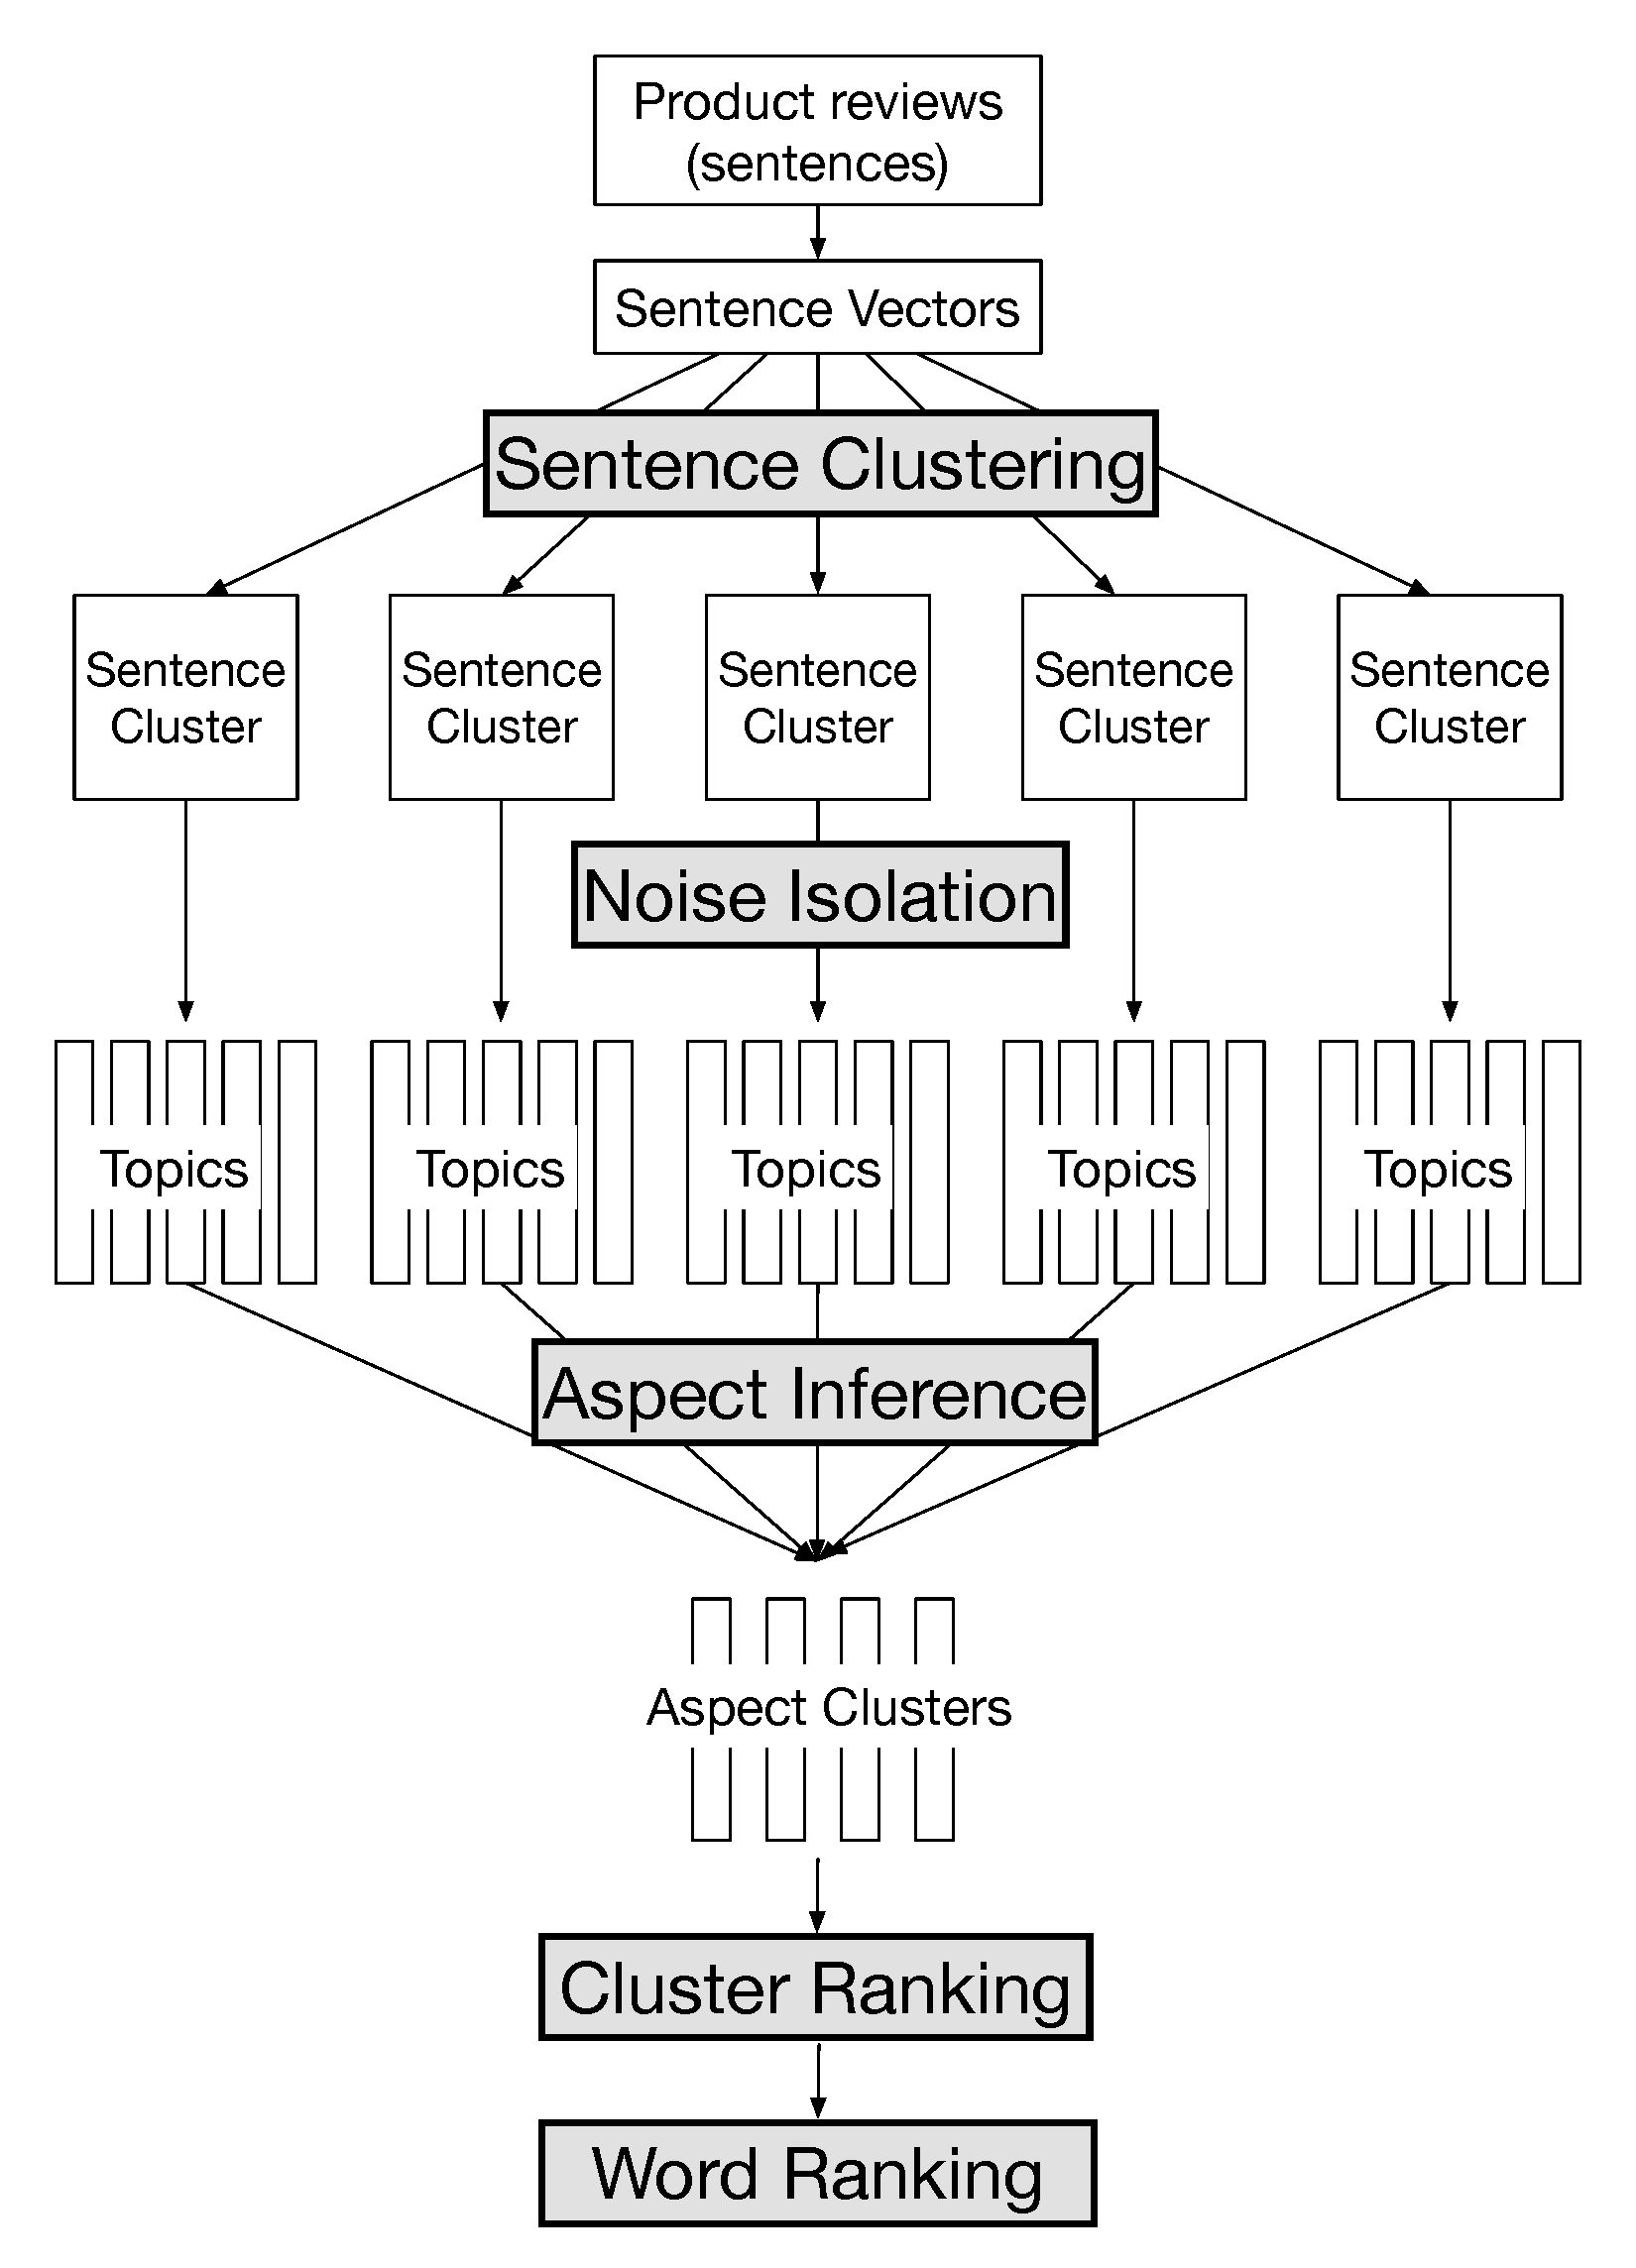
\epsfig{file=figures/framework.pdf, width=1.0\columnwidth}
	\caption{Workflow for computing the cross-cultural similarity between 
		an English word \textit{W} and a Chinese word \textit{U}, denoted by $ccsim(W, U)$}
	%\vspace{-15pt}
	\label{fig:overview}
\end{figure}


%~\footnote{There are open-sourced
%resources for these words as the following sections describe.}
%\BL{maybe use another expression for the social words} 
\subsection{Overall Workflow}
\label{sec:flow}
\figref{fig:overview} shows the workflow of our framework to construct the \textit{\socvec}~and compute $ccsim(W,U)$. 
Our proposed \textit{\socvec}~model attacks the problem with the help of three low-cost external resources: 
(i) an English corpus and a Chinese corpus from social media; (ii) an English-to-Chinese bilingual lexicon (\textit{BL});  
(iii) an English social word vocabulary (\textit{ESV}) and a Chinese one
(\textit{CSV}).

We train English and 
Chinese word embeddings (\textit{EnVec} and \textit{CnVec}) 
on the English and Chinese social media corpus respectively. 
Then, 
we build a \textit{BSL}
from the \textit{CSV}, \textit{ESV} and \textit{BL} (see~\secref{sec:bsl}). 
The \textit{BSL} further maps the previously incompatible \textit{EnVec} and \textit{CnVec} 
into a single common vector space \textit{\socvec},
where two new vectors, $S_W$ for $W$ and $S_U$ for $U$,
are finally comparable.
%
%\subsection{{SocVec} Modeling}
%\label{sec:model}
%In this section, we present the details of SocVec.

\subsection{Building the {BSL}}
\label{sec:bsl}
The process of building the \textit{BSL} is 
illustrated in~\figref{fig:BSL}. 
We first extract our bilingual lexicon (\textit{BL}), where confidence score 
$w_i$ represents the probability distribution on the multiple translations 
for each word. 
Afterwards, we use BL to translate each social word 
in the \textit{ESV} to a set of Chinese words and then filter out all the words that are not in the \textit{CSV}. 
Now, we have a set of Chinese social words for each English social word, which is denoted by a ``translation set''. 
The final step is to generate a Chinese ``pseudo-word'' for each 
English social word using their corresponding translation sets.
{A ``pseudo-word'' can be either a real word that is the most 
representative word in the translation set, or an imaginary word whose 
vector is a certain combination of the vectors of the words in the 
translation set.}

\begin{figure*}[th]
	\centering
	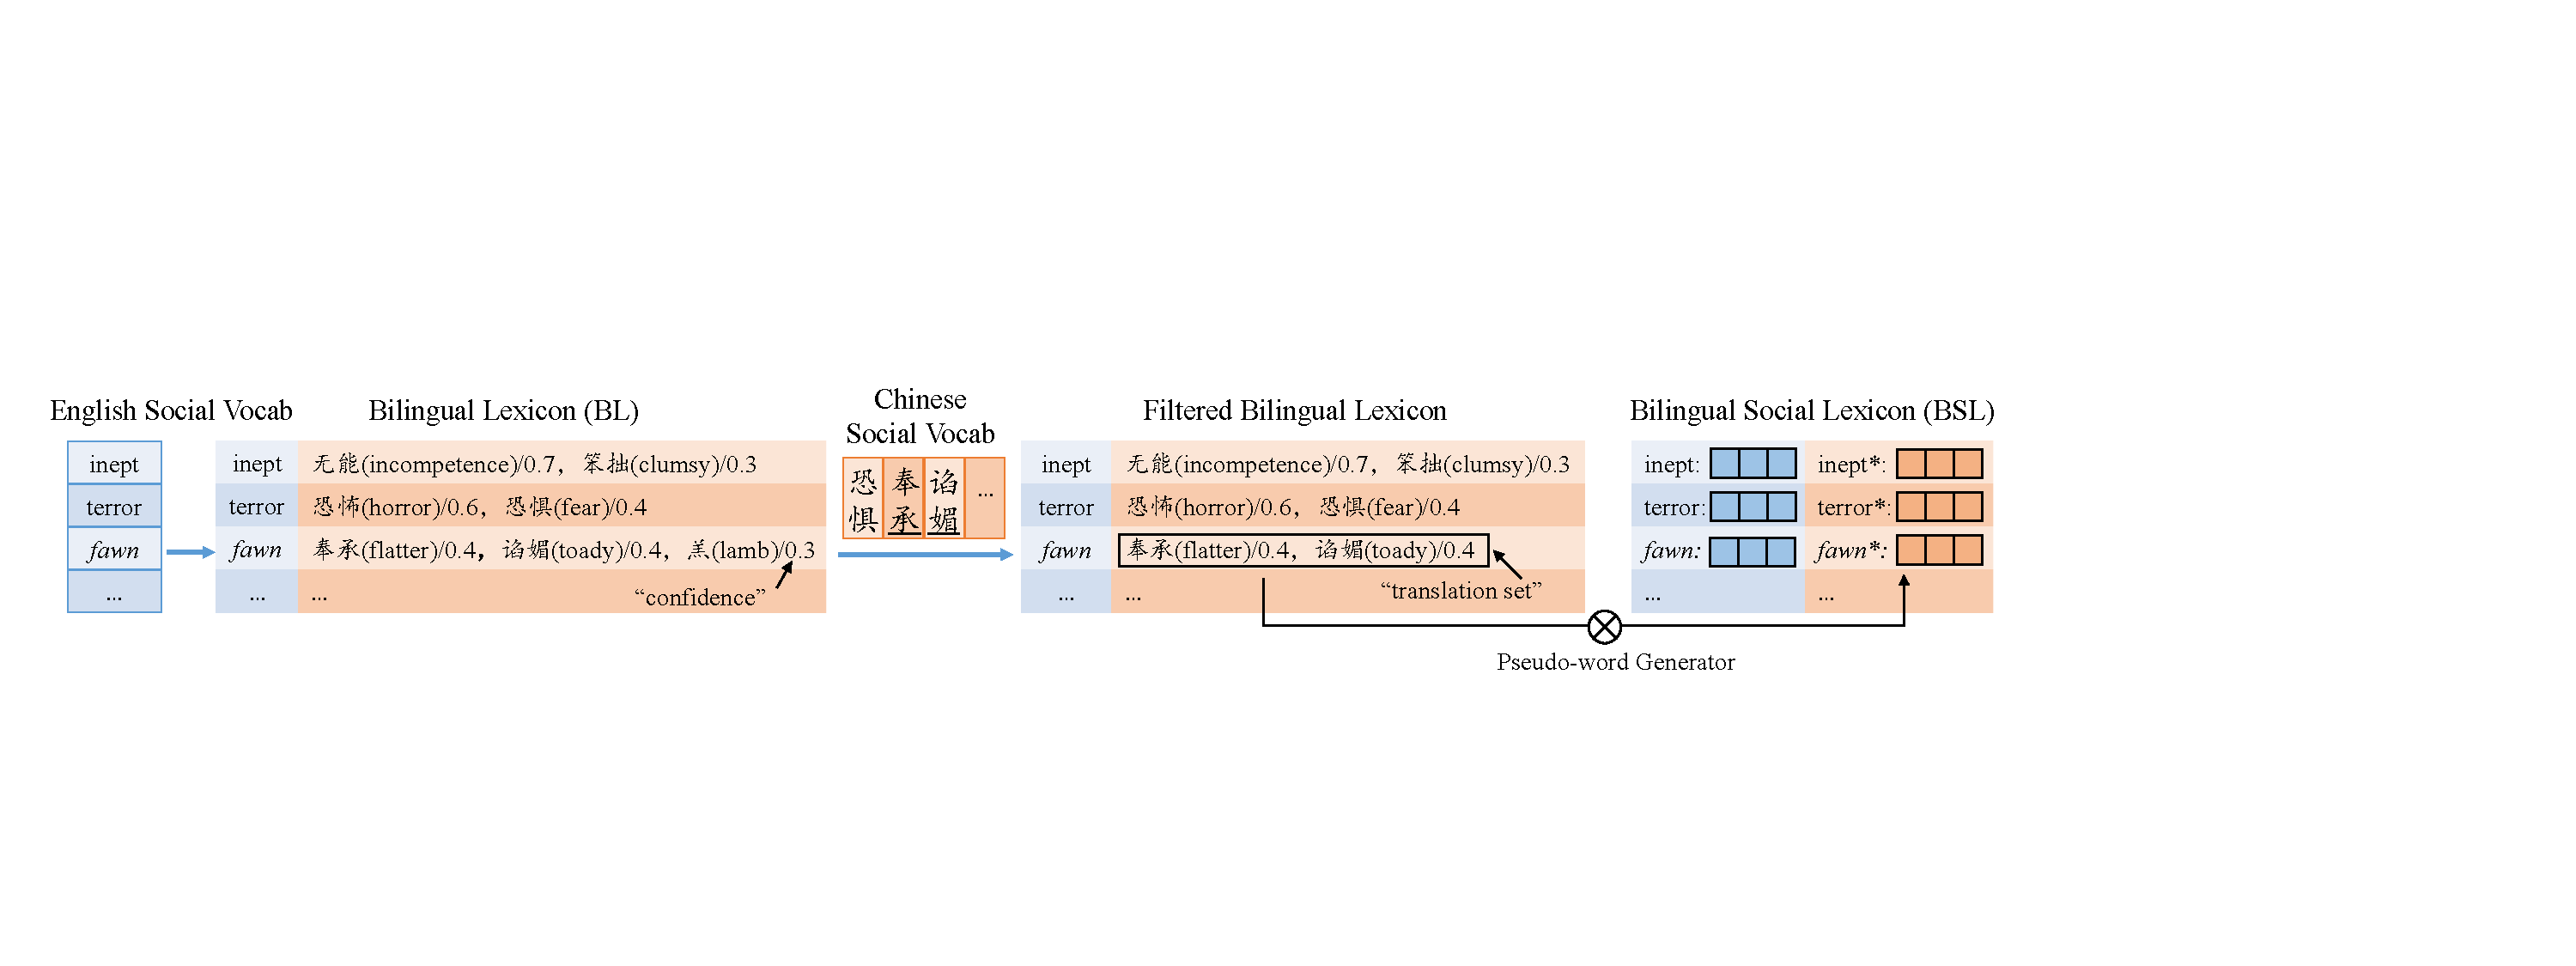
\epsfig{file=figures/bsl.pdf, width=1\textwidth}
	%	\vspace{-15pt}
	\caption{Generating an entry in the BSL for ``\textit{fawn}'' 
		and its pseudo-word ``\textit{fawn}*''}
	\label{fig:BSL}
	%	\vspace{-15pt}
\end{figure*}

For example, in \figref{fig:BSL}, the
English social word ``\textit{fawn}'' has three Chinese translations in the 
bilingual lexicon, but only two of them (underlined) are in the CSV. 
Thus, we only keep these two in the translation set in the filtered bilingual lexicon.
The pseudo-word generator takes the word vectors of the two words (in the black box), namely
奉承 (flatter) and 谄媚 (toady), as input, and generates the pseudo-word 
vector denoted by ``\textit{fawn*}''. {Note that the direction of building \textit{BSL} can also be from Chinese to English, 
	in the same manner. 
	However, we find that the current direction 
		gives better results due to the better translation quality of our \textit{BL} in this direction.}
%\footnote{The reason why we use the direction from English to Chinese  is that English socio-linguistic vocabularies tend to be more accessible and accurate than low-resource languages. The filter is optional for low-resource language which has no socio-linguistic lexicon, if we can afford the inaccuracy.}

Given an English social word, we denote $\mathbf{t_i}$ as the $i^{th}$ Chinese word of its translation set consisting of $N$ social words.
We design four intuitive types of pseudo-word generator as follows, which are tested in the experiments:

\noindent
\textbf{(1) Max.} Maximum of the values in each dimension, assuming dimensionality is $K$:
%\vspace{-10pt}
{\begin{equation*}
	\text{Pseudo}(\mathbf{C_{t_1}},...,\mathbf{C_{t_N}}) = \small \begin{bmatrix}
	max(C_{t_1}^{(1)},...,C_{t_N}^{(1)}) \\
	\vdots   \\
	max(C_{t_1}^{(K)},...,C_{t_N}^{(K)})
	\end{bmatrix}^{\rm T} \\
\end{equation*}}%
\noindent
\textbf{(2) Avg.} Average of the values in every dimension:
{$$\text{Pseudo}(\mathbf{C_{t_1}},...,\mathbf{C_{t_N}})=\frac{1}{N}\sum_i^N\mathbf{C_{t_i}} $$}

\noindent
\textbf{(3) WAvg.} Weighted average value of every dimension 
with respect to the translation confidence:
{$$\text{Pseudo}(\mathbf{C_{t_1}},...,\mathbf{C_{t_N}})=\frac{1}{N}\sum_i^Nw_i \mathbf{C_{t_i}} $$}
\noindent
\textbf{(4) Top.} The most confident translation:
{$$	\text{Pseudo}(\mathbf{C_{t_1}},...,\mathbf{C_{t_N}}) = \mathbf{C_{t_k}}, \text{} k = \argmax_i{w_i} $$}
~~Finally, the \textit{BSL} contains a set of English-Chinese word vector pairs, where each entry represents an English social word and its Chinese pseudo-word based on its ``translation set''.


\subsection{Constructing the {\socvec}~Space}
\label{sec:pg}
%\textbf{Notation Definition.} 

Let $B_i$ denote the English word of the $i^\text{th}$ entry of the \textit{BSL}, and its corresponding Chinese pseudo-word is denoted by $B_i^*$.  
We can project the English word vector $\bf{E_W}$ into the \textit{\socvec} space by 
computing the cosine similarities between $\bf{E_W}$ and each English
word vector in \textit{BSL} as values on~\socvec\ dimensions, effectively constructing a new vector $\bf{S_W}$ of size $L$. 
Similarly, we map a Chinese word vector $\bf{C_U}$ to be a new vector $\bf{S_U}$. 
$\bf{S_W}$ and $\bf{S_U}$ belong to the same vector space \textit{\socvec} 
and are comparable. The following equation illustrates the projection, and how to compute $ccsim$\footnote{{The function $sim$ is a generic similarity function, for which several metrics are considered in experiments.}}.
\begin{align*} 
&ccsim(W,U) := f(\mathbf{E_\text{W}},\mathbf{C_\text U}) \\ 
&=sim\left( 
\small{\begin{bmatrix} 
	cos(\mathbf{E_\text W},\mathbf{E_{ B_1}})\\
	\vdots \\
	cos(\mathbf{E_\text W},\mathbf{E_{B_L}})
	\end{bmatrix}^{\rm T},}
\begin{bmatrix}
cos(\mathbf{C_\text U},\mathbf{C_{B_1^*}})\\
\vdots \\
cos(\mathbf{C_\text U},\mathbf{C_{B_L^*}})
\end{bmatrix}^{\rm T}\right)\\
&=sim(\mathbf{S_\text W},\mathbf{S_\text U})  
\end{align*}
%}%
\normalsize

For example, if $W$ is ``Nagoya'' and $U$ is ``名古屋'', we compute the
cosine similarities between ``Nagoya'' and each English social word in the \textit{BSL} with their monolingual word embeddings in English.
Such similarities compose $\bf{S_{\text{nagoya}}}$. 
Similarly, we compute the cosine similarities
between ``名古屋'' and each Chinese pseudo-word, and compose the social word 
vector $\bf{S_{\text{名古屋}}}$. 

In other words, for each culture/language, the new word vectors like $S_\text W$ are constructed based on the monolingual similarities of each word to the vectors of a set of task-related words (``social words'' in our case). 
This is also a significant part of the novelty of our transformation method. 
%Bridging two cultures and languages by connecting task-related words in different languages is also 

%\scriptsize 
%	\setlength{\abovedisplayskip}{6pt}
%	\setlength{\belowdisplayskip}{\abovedisplayskip}
%	\setlength{\abovedisplayshortskip}{5pt}
%	\setlength{\belowdisplayshortskip}{5pt}
%\noindent where $cos$ denotes the cosine similarity.
%The function $sim$ is a generic similarity function, for which a number of
%metrics will be considered later in experiments.
%
%to project $\mathbf{E_W}$ and $\mathbf{C_U}$ to $\mathbf{S_W}$ and $\mathbf{S_U}$ so that they can be comparable to each other.
%We define the function $f$ to compute cross-lingual similarity between $W$ and $U$ as follows.\footnote{Here $cos$ stands for cosine similarity, } This calculation process is also shown in ~\algref{alg:alg1}. \\
%
%\begin{algorithm}[th]
%	\small
%	\DontPrintSemicolon
%	\caption{Compute cross-lingual similarity between an English word 
%		\textit{W} and a Chinese word \textit{U} } 
%	\label{alg:alg1}
%	\KwIn{ \textit{EnVec}, \textit{CnVec}, $BSL$ with $L$ word pairs} 
%	\KwOut{the cross-lingual similarity $ccsim(W,U)$} 
%	$E_W$ = word vector of $W$ in \textit{EnVec}\\
%	$C_U$ = word vector of $U$ in \textit{CnVec}\\
%	$S_W$ =  zero vector with $L$ dimension \\
%	$S_U$ =  zero vector with $L$ dimension \\
%	%	\Comment*[l]{Project $E_W$ into $S_W$}
%	\For{$1 \le i \le L$}{
%		$B_i$ =  $i^{th}$ English word in \textit{BSL} \\
%		$B_i^*$ = Chinese pseudo-word of $B_i$ \\
%		$S_W[i]$ = $cos(E_W,E_{B_i})$\\
%		$S_U[i]$ = $cos(C_U,C_{B_i^*})$\\
%	} 
%	\Return $ccsim(W,U)$ = $sim(S_W,S_U)$\\
%\end{algorithm}
%\begin{figure}[th!]
%	\centering
%	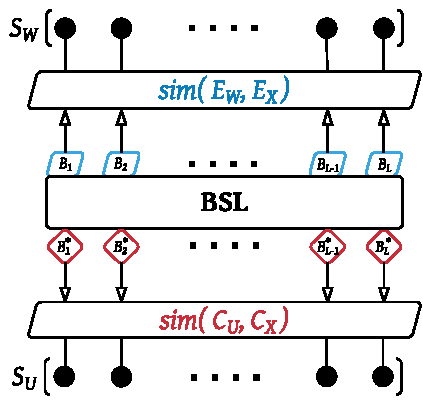
\epsfig{file=figures/SocVec.pdf, width=0.6\columnwidth}
%	\caption{Using \textit{BSL} to project $E_W$ and $C_U$ to $S_W$ and $S_U$.}
%	\label{fig:swsu}
%\end{figure}

%\subsubsection{Parameters Description}
%\label{sec:pd}
%Here, we briefly summarize the main parameters of \textit{SocVec} model:
%\begin{itemize}
%\item Two trained monolingual word embeddings, \textit{EnVec} and \textit{CnVec};  
%\item A bilingual lexicon;
%\item Chinese and English socio-linguistic vocabularies; 
%\item Pseudo-word generator function; 
%\item Option of similarity function $sim$; 
%\end{itemize} 
%We conduct several experiments for testing the these parameters in~\secref{sec:mcdne}.

\subsection{Mining Cross-cultural Differences of Named Entity}
\label{sec:mcdne}
This task is to discover and quantify cross-cultural differences of concerns towards name entities. 
We first explain how we obtain the ground truth from human annotators, then present several baseline methods to this problem and finally 
show our experiment results in detail.

\subsubsection{Ground Truth}
\label{sec:mcdne_truth}
Harris~\shortcite{harris1954distributional} states that the meaning of 
words is evidenced by the contexts they occur with. 
Likewise, in this work, we assume that the cultural properties of an entity 
can be captured by the terms they co-occur with in large text corpus. 
Thus, for each named entity, we present four human annotators\footnote{All four annotators are native Chinese speakers but bilingual. Two of them lived in the US extensively.} with two lists of 20 most co-occurred words with 
the named entity, from Twitter and Weibo respectively. 
We select 700 named entities for annotators to label, which
are the most frequently mentioned both in Twitter and Weibo. 
Annotators are instructed to rate the relatedness between the 
two word lists with one of following labels: ``very different'', 
``different'', ``hard to say'',  ``similar'' and 
``very similar''.\footnote{Our annotators are educated with many 
selected examples and thus have shared understanding of the five-level 
labels. Ranking based annotation method demands annotators to look 
at 40+40 words for the two terms in two languages before a decision can
be made, which is more expensive and harder to administer in our opinion.}

We then map the labels to numerical scores from 1 to 5
and use the average scores from the annotators as the ground truth 
for score ranking and binary classification.
For the binary classification problem, 
an entity is considered culturally similar 
if the score is larger than 3.0, and culturally different otherwise.
The inter-annotator agreement is 0.672 by Cohen's kappa coefficient, 
suggesting substantial correlation, according to the Wikipedia entry
of Cohen's kappa.
%\BL{ (0.531 without hanyuan)}

\subsubsection{Baselines and Our Method}

We propose five baseline methods. The first three
\emph{distribution}-based, while the next two 
are \emph{transformation}-based. 
Distribution-based methods compare the lists of surrounding
English and Chinese terms, denoted as $L_E$ and $L_C$, 
by computing the cross-lingual relatedness between the two lists, 
though different baselines differ by the
selection of words and the way similarity is computed.
Transformation-based methods compute the vector representation 
in English and Chinese corpus respectively, and
then trains a transformation.
% of words, known $L_E$ and $L_C$. The differences of these methods are the selecting method of terms and %the computation method of two word lists.  ii) the second type of baseline methods are first obtain the %comparable vectorial representation of the English title and Chinese title of the given entity, and then just %calculate the similarity between two comparable vectors.

\textbf{Bilingual Lexicon Jaccard Similarity (BL-JS)}
%	The $L_E$ and $L_C$ of both BL-JS and WN-WUP  are the same as the lists that annotators judge.
BL-JS uses the bilingual lexicon to translate $L_E$  to a Chinese word list 
$L_E^*$ as a medium and then calculates the Jaccard Similarity between 
$L_E^*$ and $L_C$ as $J_{EC}$. Similarly, we can compute $J_{CE}$. 
Finally, we compute $\frac{J_{EC}+J_{CE}}{2}$ as the cross-cultural similarity 
of this given name entity.
 
	\textbf {WordNet Wu-Palmer Similarity (WN-WUP)} Instead of using 
the bilingual lexicon and Jaccard Similarity, WN-WUP uses Open Multilingual 
Wordnet~\cite{wang2013building,bond2013linking} to calculate the average 
similarity of two lists of words from different languages.
	
	\textbf {Word Embedding based Jaccard Similarity (EM-JS)} EM-JS is 
very similar to BL-JS, except that its $L_E$ and $L_C$ are generated by 
ranking the similarities between the name of entities and all English words 
and Chinese words respectively. 

	\textbf {Linear Transformation (LTrans)}
	We follow the steps in Mikolov et al.~\shortcite{Mikolov:2013tp} 
to train a transformation matrix between \textit{EnVec} and \textit{CnVec}, 
using 3000 translation pairs with confidence of 1.0 in the bilingual lexicon. 
Given a named entity, this solution simply calculates cosine similarity 
between the vector of its English name and the \textit{transformed} vector 
of its Chinese name. 
	
	\textbf {Bilingual Lexicon Space (BLex)}
	This baseline is similar to \textit{SocVec} but it does not 
utilize socio-linguistic vocabularies and simply uses the bilingual lexicon
as the BSL.

\textbf{{Our SocVec-based method}} Given a named entity with its English and 
Chinese name, we simply compute the similarity between their 
\textit{SocVec}s as its cross-cultural difference score. 

\subsubsection{Experimental Results}

For qualitative evaluation, \tabref{tab:mcdne_res_4} shows some of 
the most culturally different entities obtained by our method. 
The hot and trending topics on Twitter and Weibo are 
manually summarized to help explain the cultural difference. 
All listed entities have large divergence on concerns, 
thus reflecting cross-cultural differences.
\begin{table*}[th!]
	\footnotesize
	\centering
	\caption{{Selected culturally different named entities, with Twitter and Weibo's trending topics manually summarized}}
	\begin{tabular}{|L{1.5cm}|L{5cm}|L{8cm}|}
		\hline
		\textbf{Entity} & \textbf{Twitter topics} & \textbf{Weibo topics}
		\\ \hline
		Maldives & coup, president Nasheed quit, political crisis & holiday, travel, honeymoon, paradise, beach \\ \hline
		Nagoya & tour, concert, travel, attractive, Osaka & Mayor Takashi Kawamura, Nanjing Massacre, denial of history\\  \hline
%		Quebec & Conservative Party, Liberal Party, politicians, prime minister, power failure & travel, autumn, maples, study abroad, immigration, independence   \\ \hline
%		Philippines & gunman attack, police, quake, tsunami & South China Sea, sovereignty dispute, confrontation, protest  \\ \hline
		Yao Ming & NBA, Chinese, good player, Asian  & patriotism, collective values, Jeremy Lin, Liu Xiang, Chinese Law maker, gold medal superstar   \\ \hline
		University of Southern California & college football, baseball, Stanford, Alabama, win, lose & top study abroad destination, Chinese student murdered, scholars, economics, Sino American politics \\ \hline
	\end{tabular}
	\label{tab:mcdne_res_4}
\end{table*}

\begin{table}[th]
	\small
	\centering
	\caption{{Comparison of Different Methods}}
	\begin{tabular}{|l|c|c|c|}
		\hline
		\textbf{Method} & \textbf{Spearman} & \textbf{Pearson}  & \textbf{MAP} \\ \hline\hline
		BL-JS& 0.276 & 0.265 & 0.644   \\ \hline
		WN-WUP  & 0.335 & 0.349 & 0.677 \\ \hline
		EM-JS & 0.221 & 0.210  & 0.571\\ \hline
		LTrans& 0.366 & 0.385  & 0.644  \\ \hline
		BLex& 0.596 & 0.595  & 0.765 \\ \hline\hline
		SocVec:opn& 0.668 & 0.662   & \textbf{0.834} \\ \hline
		SocVec:all& \textbf{0.676} & \textbf{0.671}  & \textbf{0.834}\\ \hline
	\end{tabular}
	\label{tab:mcdne_res_1}
\end{table}
\begin{table}[th]
	\centering
	\small
	\caption{{Evaluation of Different Similarity Functions}}
	\label{tab:mcdne_res_2}
	\begin{tabular}{|l|c|c|c|}
		\hline
		\textbf{Similarity} & \textbf{Spearman} & \textbf{Pearson}   & \textbf{MAP} \\ \hline\hline
		PCorr. & 0.631 & 0.625 & 0.806\\ \hline
		L1 + M & 0.666 & 0.656 & 0.824 \\  \hline
		Cos & \textbf{0.676} & 0.669 & \textbf{0.834} \\ \hline
		L2 + E & \textbf{0.676} & \textbf{0.671} & \textbf{0.834} \\ \hline
	\end{tabular}
\end{table}

\begin{table}[th]
	\centering
	\small
	\caption{{Evaluation of Different Pseudo-word Generators}}
	\begin{tabular}{|l|c|c|c|}
		\hline
		\textbf{Generator} & \textbf{Spearman} & \textbf{Pearson}   & \textbf{MAP} \\ \hline \hline
		Max. & 0.413 & 0.401 & 0.726\\ \hline
		Avg. & 0.667 & 0.625 & 0.831\\ \hline
		W.Avg. & 0.671 & 0.660 & 0.832 \\  \hline
		Top & \textbf{0.676} & \textbf{0.671} & \textbf{0.834} \\ \hline
	\end{tabular}
	\label{tab:mcdne_res_3}
\end{table}

In~\tabref{tab:mcdne_res_1}, we evaluate the baseline methods and 
our approach with three metrics: Spearman and 
Pearson correlation on the ranking problem, and Mean Average Precision (MAP)
on the classification problem (see \secref{sec:mcdne_truth}). The \textit{BSL} of \textit{SocVec:opn} uses only OpinionFinder as English socio-linguistic vocabulary, while \textit{SocVec:all} uses the union of Emapth and OpinionFinder vocabularies.\footnote{
Having tuned the  parameters, we use the best parameters for the \textit{SocVec:opn} method and \textit{SocVec:all} method: 
monolingual word vectors are trained with 5-word context window and 150 dimensions;
choosing cosine similarity as the \textit{sim} function to compute the similarity within the \textit{\socvec}~space;
using ``\textit{Top}'' pseudo-word generator
(see \secref{sec:model}).
} Results show that \textit{SocVec} models perform the best and 
using the union of vocabularies is better.

We also evaluate the effect of four different similarity options in 
\textit{\socvec}, namely, Pearson Correlation Coefficient 
(\textit{PCorr}.), L1-normalized Manhattan distance (\textit{L1+M}), 
Cosine Similarity (\textit{Cos}) and  L2-normalized Euclidean distance (\textit{L2+E}).
%It is mathematically proved that \textit{L2+E} is identical to \textit{Cosine} in ranking.
From~\tabref{tab:mcdne_res_2}, we conclude that among these four options, \textit{Cos} and \textit{L2+E} perform the best. 
%Although it is mathematically proved that \textit{L2+E} is identical to \textit{Cosine} in ranking, we can find that 
\tabref{tab:mcdne_res_3} shows effect of using four different 
pseudo-word generator functions (see~\secref{sec:pg}), from which we can infer that ``\textit{Top}'' generator function performs best for 
it reduces the noise brought by the less possible translation pairs. 


\section{Task 2: Finding most similar words for slang terms across languages}
\label{sec:bleis}
%In this section, we evaluate our model on the second task, which   
%In this section, we first introduce the ground truth and baseline methods for comparison. Then, we analyze the experimental results quantitatively and qualitatively.
\textbf{Task Description:} This task aims to find the most similar English words in terms of meaning and sentiment of a given Chinese slang term, or vice versa. The input is a list of English (or Chinese) slang terms of interest and two monolingual social media corpora; the output is a list of Chinese (or English) word sets with respect to each input slang term.
Simply put, for each given slang term, we aim to find a set of the words (in the other language) that are most similar to it and thus can help people understand it across languages.
We propose using Average Cosine Similarity (see~\secref{sec:exp}) to evaluate each method's output with ground truth word sets (presented below).

\subsection{Ground Truth}
\textbf{Slang Terms}
We collect our Chinese slang terms from an online Chinese slang glossary\footnote{\scriptsize{\url{https://www.chinasmack.com/glossary}}} consisting of 200 popular slang terms with English explanations. 
For English, we resort to a slang word list from OnlineSlangDictionary\footnote{\scriptsize{\url{http://onlineslangdictionary.com/word-list/}}} with explanations and downsample the list to 200 terms.
%To evaluate the performance of our model, 
%we propose to build the ground truth based on above-mentioned explanations from the glossary and slang dictionary. 
%Since the subtle and latent semantics of slang are too difficult to translate without losing any information, exact translation are always missing.

\noindent
\textbf{Truth Word Sets}
For each Chinese slang term, its truth English word set is hand picked from the English explanation in the glossary. 
For example, we construct the ground truth target terms for 
the Chinese slang term ``二百五'' by manually labeling words related to its meaning in the glossary:
~\\ \vspace{-5pt}
\begin{description}
	\item[二百五:] A \textbf{\textit{foolish}} person who is lacking in sense but still \textbf{\textit{stubborn}}, \textbf{\textit{rude}}, and \textbf{\textit{impetuous}}.
\end{description}

\noindent
Similarly, for each English slang term, its  Chinese word sets are the translation of the words hand picked
from its English explanation.
%Different methods should produce a list of translation terms 
%as similar as possible to the ground truth target terms.

%and then computing the average similarity between the source term and the target terms is a better approach to evaluate a bilingual slang lexicon induction system.



%what are the good word translation that best preserve and convey the meaning, sentiment tendency and usage context ot the original slang. 
%However most of the slangs possess most subtle senses that are related to native culture background, general characteristic and language style of netizens in different language worlds. 
%Thus it is really difficult, if not impossible, to find a exact word in another language that carries the exact same meaning with the original slang. 
%Because of this, our ground truth does not pursue exact Internet slang translation from one language to another's corresponding slang, since most likely such slang does not exist yet. 
%Our aim for the task is using IV (in-vocabulary) normal related words in target language to describe and translate the OOV (out-of-vocabulary) slang words in another language, which is more viable and feasible, and easier for people in different culture/language to understand not just literal meaning but the deeper buried and more subtle sense and context it conveys.
%
%Following this goal, we could build our ground truth based on filtered glossary. For Chinese slangs, we tokenize and lemmatize the definition sentences in English and manually remove the stop words that does not contribute to the meaning of a specific slang, left with a list of English words that have either same meaning or high relatedness to the Chinese slang.
%The same process is applied to English slang glossary as well, with the only difference is that due to the lack of direct Chinese definitions, we have to use Google Translate to translate the definition sentences to Chinese and human annotators tokenize, filter and paraphrase the definitions into Chinese word lists, resulting in the ground truth of slangs in the same format as the Chinese ones.
%Note that we do not manually add word translations by ourselves, we only delete irrelevant words for later evaluation, thus lowering the human error, cross-cultural and bilingual requirement to the minimum.

\begin{table*}[th!]
	\scriptsize
	\centering
	\caption{\small Slang Translation Examples \vspace{-10pt}}
	\begin{tabular}{L{1.2cm}|L{4.7cm}|L{1.7cm}|L{1.7cm}|L{1.7cm}|L{2.8cm}}
		\textbf{Slang} & \textbf{Explanation} & \textbf{Google}& \textbf{Bing}& \textbf{Baidu} & \textbf{Ours} \\ \hline 
		浮云 &something as ephemeral and unimportant as ``passing clouds''& clouds& nothing& floating clouds & nothingness, illusion \\ \hline
		水军 &``water army'', people paid to slander competitors on the Internet and to help shape public opinion& Water army& Navy& Navy & propaganda, complicit, fraudulent\\ \hline
		%		城管 & ``City administrators'', who enforce city regulations, with poor reputation as being corrupt and violent, best known for physically bullying illegal street peddlers & urban management& urban management& urban management & terrorist, rioting, threaten\\ \hline \hline
		floozy & a woman with a reputation for promiscuity & N/A&劣根性 (depravity)&荡妇(slut)&骚货(slut),妖精(promiscuous)\\ \hline
		fruitcake& a crazy person, someone who is completely insane & 水果蛋糕 \quad(fruit cake)&水果蛋糕 \qquad(fruit cake)&水果蛋糕 \quad(fruit cake)& 怪诞(bizarre),厌烦(annoying)\\ \hline
		%		nonce &  A person convicted (or simply guilty) of sexual crimes, especially pedophilia. Or a common British insult regardless of the tendencies of the person &随机数 (random numbers)&杜撰 (fabricate)&杜撰 (fabricate) & 伤风败俗(immoral),十恶不赦(extremely evil),畜类(beast),令人发指(heinous)\\ \hline
	\end{tabular}
	\label{tab:bleis_3}
\end{table*}
\subsection{Baseline and Our Methods} 
We propose two types of baseline methods for this task. 
The first type is based on well-known {\em on-line translators}, 
namely Google (Gg), 
Bing (Bi) and Baidu (Bd).\footnote{Experiments using them are done in August, 2017.}  
%With our test set's slang as input, we retrieve the output of translation. 
Another baseline method for Chinese is  CC-CEDICT\footnote{\scriptsize{\url{https://cc-cedict.org/wiki/}}} (CC), an on-line public-domain Chinese-English dictionary, which is constantly updated with popular slang terms. 

Considering situations where many slang terms have literal meaning as well, it may be unfair to retrieve target terms from such on-line translators by solely inputing slang terms without slang contexts. 
Thus, we utilize example slang-meaning sentences from some websites (mainly from Urban 
Dictionary\footnote{\scriptsize{\url{http://www.urbandictionary.com/}}}) 
%as input to them, so that the translators have a greater chance of knowing this is a slang use, rather than an ordinary term. \footnote{Nevertheless, we noticed
%that on-line translators often cannot capture such slang contexts and still produce literal translations.}
The following example using Google Translation shows how we obtain the target translation terms for the slang word ``fruitcake'' (an insane person) from Google Translator:
{\textit{Oh man, you don't want to date that girl. She's always drunk and yelling. She is a total \underline{\textbf{fruitcake}}.}}\footnote{\scriptsize{\url{http://www.englishbaby.com/lessons/4349/slang/fruitcake}}} 
\textit{Google Translation:}
{\small哦, 男人, 你不想约会那个女孩。她总是喝醉了, 大喊大叫。她是一个\underline{\textbf{水果蛋糕}}。}

%Since all possible target terms come from the bilingual lexicon, 
Another lines of baseline methods is ranking based.
We can score each of them in our bilingual lexicon and consider the top K words as the target terms. 
Given a source term to be translated, several such {\em scoring-based baseline methods} are as follows.
Linear Transform (LT), MultiCCA, MultiCluster and Duong method score the candidate target terms by 
computing cosine similarities in their constructed bilingual vector space with the tuned best settings in previous evaluation. 
A more sophisticated baseline (TransBL) leverages the bilingual lexicon: 
for each candidate target term $w$, we first obtain its translations 
$T_w$ back into the source language and then calculate the average word similarities between the source term and $T_w$  as the score of $w$. 
%Now over 20,000 words in the other language of the bilingual lexicon have their corresponding similarity score to the given slang. 
%A word may have multiple possible translation words in the other language. In this case, we choose to take average over all of them in terms of similarity score.
%We then rank the words by their scores and take top 5 words to form a word set, while other online translation baselines directly produce a word set for later comparison with the ground truth word set. 
Our {\em SocVec-based method} (\textbf{SV}) simply calculates the cosine similarities between the source term and each candidate target term within \textit{\socvec} space as scores.


\begin{table}[th!] 
	\scriptsize
	\centering
	\begin{subtable}[h]{\columnwidth}
		\centering
		\begin{tabular}{|ccccc|}
			\hline
			Gg&  Bi& Bd & CC & LT   \\ 
			18.24 &  16.38&  17.11 & 17.38 & 9.14 \\ \hline   
			TransBL& MultiCCA & MultiCluster & Duong   & SV \\ 
			18.13 &  17.29 & 17.47&  20.92& \textbf{23.01}\\ \hline  
		\end{tabular}
		\subcaption{Chinese Slang to English}
	\end{subtable}
	\vfill \hfill
	\begin{subtable}[h]{\columnwidth}
		\centering
		\begin{tabular}{|ccccc|}
			\hline
			Gg&  Bi& Bd &  LT   & TransBL\\ 
			6.40  &   15.96 &  15.44  & 7.32 & 11.43\\ \hline   
			MultiCCA & MultiCluster & Duong   & SV & \\ 
			15.29 & 14.97&  15.13& \textbf{17.31} & \\ \hline  
		\end{tabular}
		\subcaption{English Slang to Chinese}
	\end{subtable}
	\caption{\small ACS Sum Results of Slang Translation \vspace{-5pt}}
	\label{tab:bleis_acs}
\end{table}
\subsection{Experimental Results}
\label{sec:exp}
To quantitatively evaluate our methods, we need to measure similarities between the produced target term set and the ground truth word set. 
Exact-matching Jaccard similarity is too strict to capture valuable relatedness between two word sets.
We argue that average cosine similarity (ACS) between two sets of word vectors is a better metric to evaluate the similarity between two word sets. The following equation illustrates such computation, where $A$ and $B$ are the two word sets, $\mathbf{A_i}$ and $\mathbf{B_j}$ denotes the word vector of the $i^{th}$ word in $A$ and $j^{th}$ word in $B$ respectively. 
The word vectors used in ACS computation is a third-party pre-trained 
embedding\footnote{\scriptsize \url{https://nlp.stanford.edu/projects/glove/}} and thus the ACS computation is fair over different methods.
Table 6 shows the sums of ACS over 200 slang translations. 
\begin{align*}
ACS (A,B)=
{\frac{1}{|A||B|}}{\sum_{i=1}^{|A|}{\sum_{j=1}^{|B|}} \frac{\mathbf{A_i }\cdot \mathbf{B_j}}{\|\mathbf{A_i }\|\|\mathbf{B_j }\|}}
\end{align*}


Experimental results of Chinese and English slang translation in terms of the sum of \textit{ACS} over 200 terms are shown in~\tabref{tab:bleis_acs}.
The performance of on-line translators for slang typically depends on human-set rules and supervised learning on well-annotated parallel corpora, which are rare and costly, especially for social media where slang emerges the most. This could be a possible reason why they do not perform well. 
Linear transformation model is trained on translation pairs with high confidence in the bilingual lexicon, which contains little information about the OOV slang terms and social context on them, which is why LT method performs badly.
\textit{BL} method is competitive because its similarity computations 
are within monolingual semantic spaces and it uses a bilingual lexicon 
to transform, while it loses the information from the related words 
which are not in the bilingual lexicon.
%Experiment results of Chinese and English slang translation in terms of the sum of \textit{ACS} over the translations of 200 slang terms are shown in~\tabref{tab:bleis_acs}.
%The performance of online translators for slang terms typically depends on human-set rules and supervised learning on well-annotated parallel corpora, which are rare and costly, especially for social media where Internet slang emerges the most. 
%This could be a possible reason why they do not perform well. 
%~Linear transformation model is trained on translation pairs with high confidence in the bilingual lexicon, which contains little information about the OOV slang terms and social context on them, which is the reason why  LT method performs badly.
%\textit{BL} method is competitive for its similarity computations are within monolingual word vector spaces and uses a bilingual lexicon to transform, while it loses the information from the related words which are not in the lexicon translation pairs.
Our method (SV) outperforms baselines by directly using the distances in 
our proposed bilingual embeddings~\textit{SocVec}, which proves 
that ~\textit{SocVec} can capture the cross-cultural similarities between terms.
%utilizes comparable English and Chinese social media corpora and 
%encodes the context and usage of a given slang term by computing its similarities with words in the socio-linguistic vocabulary of the source language. Therefore, 
%our model keeps the cross-cultural socio-linguistic features, which is a most important reason why we outperform baselines.
%the best among all the baseline methods. 
%Then, we are able to find the most similar counterparts in the target language by computing the similarity in \textit{SocVec} space through \textit{BSL}. 
%Therefore, our performance is better than the others.    

To qualitatively evaluate our model, in~\tabref{tab:bleis_3}, 
we present several examples of our translations for Chinese and English slang 
terms as well as their explanations from glossaries.
Our results are highly correlated with these explanations and 
capture their core semantics, whereas most online translators just offer 
literal translatation of such slang terms, even with the ample
slang contexts.
% They often offer just literal meanings as translation even with the specific slang context using the example sentences from Urban Dictionary.

Additionally, we take a step forward to directly translate between 
English slang terms and Chinese slang terms by simply filtering out 
ordinary (non-slang) words in the original target term lists. 
Examples are shown in~\tabref{tab:bleis_4}. 
\begin{table}[t]
	\scriptsize
	\centering
	\caption{\small{Slang-to-Slang Translation Examples}\vspace{-10pt}}
	\begin{tabular}{C{1.92cm} C{2.5cm} C{2.0cm}}
		\textbf{Chinese Slang} & \textbf{English Slang} & \textbf{Explanation} \\ \hline
		萌 & adorbz, adorb, adorbs, tweeny, attractiveee & cute, adorable \\ \hline
		二百五 & shithead, stupidit, douchbag & A foolish person\\ \hline
		鸭梨 & antsy, stressy, fidgety, grouchy, badmood & stress, pressure, burden \\ \hline
	\end{tabular}
	\label{tab:bleis_4}
\end{table}

\section{Related Work}
\paragraph{Clarification Question Generation} The concept of CQ can be naturally raised in a dialogue system where the speech recognition results tend to be erroneous so that we raise CQs for sanity check \citep{stoyanchev2014towards}, or the intents for a task is incomplete or ambiguous in a first short utterance and further CQs are needed to fill in the slots \citep{dhole2020resolving}. The concept is then extended to IR to clarify ambiguous queries \citep{aliannejadi2019asking}, and has been successfully put into practice \citep{zamani2020generating}. Other application areas including KBQA \citep{xu2019asking} and open-domain dialogue systems \citep{aliannejadi2020convai3}. CQGen can also be applied to help refine posts on websites like StackExchange \citep{Kumar_2020} and Amazon \citep{rao2019answer}. In this context, our work closely follows the research line of \citep{rao2018learning, rao2019answer, cao2019controlling}. \citet{rao2018learning} first adopted a retrieval-then-rank approach. They \citep{rao2019answer} then proposed a generation approach to train the model to maximize the utility of the hypothetical answer for the questions with GAN, to better promote specificity. \citet{cao2019controlling} propose to control the specificity by training on data with explicit indicator of specificity, but it requires additional specificity annotation. Towards the similar specificity goal, we adopted a different keyword-based approach. They also assume generating one question per context, which we claim is not sufficient to cover various possible information needs, and thus propose the task of the diverse CQGen.

\paragraph{Diverse Generation} The demand for diverse generation exists in many other fields~\cite{vijayakumar2018diverse, LiangZ18code, shen2019mixture}, and we've drawn inspirations from these literatures. For image captioning, we may use multiple descriptions for different focusing points of a scene. \textit{Diverse Beam Search} \citep{vijayakumar2018diverse} was proposed to broaden the searching space to catch such diversity by dividing groups in decoding and imposing repetition penalty between them. For machine translation, a context can be translated with different styles. \citet{shen2019mixture} thus proposed \textit{Mixture of Expert} models including hMup to reflect various styles with a discrete latent variable (\textit{expert}). And here for CQGen, diversity is required to cover various potentially missing aspects, so we come up with the idea to use keywords as a controlling variable like \textit{expert} to promote diversity.


%\section{Future Work}
%%To this end, we have successfully built a system
%%which can solve the top-$k$ extraction problem
%%with adequate accuracy and efficiency.
%%With the big data experiment result,
%%we have built a top-$k$ database with
%%over 1.7 million top-$k$ lists of 92.0\% precision.
%%In the future, we will mainly focus on three aspects of work.
%
%The first One is to further enrich the top-$k$ database
%and improve its quality. On the one hand,
%we can use larger training data and
%more sophisticated machine learning models to
%upgrade the system performance;
%on the other hand, we can explore the other source
%of top-$k$ lists rather than top-$k$ pages.
%The slide-show pages can be a good candidate (e.g. Fig. \ref{fig:slideshow}),
%as the top-$k$ list spans across a set of pages, which are connected one another
%by hyperlinks. Intuitively, we can develop a crawler that goes through
%``Previous'' and ``Next'' links and obtain a slide-show page chain.
%But the main challenge is we can not run it on big data as the web snapshot
%cannot support random access (access by URL).
%Furthermore, the snapshot may lose some nodes in a page chain,
%thus we cannot extract the complete list.
%
%The second is to further understand top-$k$ lists, especially the top-$k$ titles.
%In Section \ref{sec:problem}, we define a function $tr$ to convert a textual title
%into a five-tuple representation, which is implemented by Title Classifier.
%However, this representation remains rough as we miss some modifiers other than time and location.
%For example, ``top 10 NBA players alive'' is different from ``top 10 NBA players who have a ring'',
%but they will share the same representation. We may need to include those modifiers in the representation,
%and redefine $tr$ as $tr : (t, d) \rightarrow \mathcal{R} = (k, c, \alpha,
%\mathcal{M})$ where $\mathcal{M}$ is a set of modifiers including the temporal modifier $\tau$ and
%spatial modifier $\sigma$. To do this, we need to improve our Title Classifier to recognize general modifiers,
%probably using the same technology.
%A harder challenge is to calculate semantical similarity between $\mathcal{R}$.
%%which can be defined as $sim : (\mathcal{R_1}, \mathcal{R_2}) \rightarrow score$.
%To solve this, we need to find out the similarity of each part
%($sim_c(c_1, c_2)$, $sim_\alpha(\alpha_1, \alpha_2)$ and $sim_\mathcal{M}(\mathcal{M}_1, \mathcal{M}_2)$)
%and develop a equation/model $sim : (sim_c, sim_\alpha, sim_\mathcal{M}) \rightarrow score$.
%With this function, we can cluster the top-$k$ lists into groups of similar semantics.
%
%The last is to utilize the top-$k$ database.
%As we discuss in Section \ref{sec:intro},
%we attempt to build a Q/A system.
%%which,
%%according to different type of queries,
%%return an instance (e.g. ``Who is the second tallest building in Beijing'') or
%%a ranked list (e.g. ``top 10 richest people in 2010'').
%Given a query $q$, we can first parse it into the tuple representation $\mathcal{R}_q=(k_q,...)$ and
%find a most similar group $g$ from the database.
%To generate a $k_q$-items ranked list (or the $k_q$th item) from $g$, there are two possible solutions.
%The list-wise approach is to (1) rank the lists in $g$ which contain more than $k_q$ items,
%and (2) return the first $k_q$ items (or the $k_q$th item) of the best list.
%The item-wise approach is to merge top-$k$ lists in a group into a bigger one,
%where the main challenge is to calculate the ranking score of each item over aggregation (of ranked lists)
%as an item can exists in multiple top-$k$ lists with different position(ranking within the list).
%This problem is popular in the area of top-$k$ query processing
%as some algorithms are proposed to solve it in different scenarios
%\cite{angel2009ranking,chakrabarti2006ranking,bansal2008ad}.
%In general, we need
%
%
%To obtain the ranking score of each item $i$,
%we need to calculate the score $s_i$ wrt. each list $L_i$ that contains $i$
%(which should be a function of item position $p_i$ and the list size $|L_i|$).
%
%
%We can first define a function $rp: (k, n) \rightarrow score$,
%which gives the score of the $n$th item in any top-$k$ list.
%Then for a instance $i$, assuming it
%
%
%%.
%%The main challenge is to calculate the ranking of each item over aggregation of lists,
%%while a similar problem in the area of top-$k$ query processing
%
%For a list item $i$, it may appears in different list $L$
%The final solution may be a hybrid of the two approach above.



\section{Conclusion}
\label{sec:conclusion}
This paper presents a novel and interesting problem of extracting
top-$k$ lists from the web.  Compared to other structured data,
top-$k$ lists are cleaner, easier to understand and more
interesting for human consumption, and therefore are an important
source for data mining and knowledge discovery. We demonstrate a
algorithm that automatically extracts over 1.7 million such lists from
the a web snapshot and also discovers the structure of each list.  Our
evaluation results show that the algorithm achieves 92.0\% precision
and 72.3\% recall.

%\ZZX{
%In the future, we will focus on building a Q/A system based on
%the large number of top-$k$ lists we extracted.
%%According to different type of queries,
%%the system should return
%%a $k$-item ranked list or the $k$th instance, where $k$ is specified in the query.
%As a top-$k$ query processing system, 
%the main challenge lies in how to generate a $k$-item ranked list 
%from all top-$k$ lists that matches the query.
%Basically we can return the first $k$ items from the best-matching list 
%that contains more than $k$ items.
%A more complicated approach is to merge top-$k$ lists in a group into a bigger one,
%where we need to calculate the ranking score of each item over aggregation (of ranked lists)
%\cite{fagin2001optimal,angel2009ranking,chakrabarti2006ranking}.
%The final solution may be a hybrid of the two approaches above.
%}
%
%Ideally, we should first cluster the top-$k$ lists into groups of similar semantics
%and find out the group $g$ that match the query best.
%To generate a $k$-items ranked list (or the $k$th item) from the group, there are two possible solutions.
%The list-wise approach is to rank the lists in $g$ which contain more than $k$ items,
%and return the first $k$ items (or the $k$th item) of the best list.
%The item-wise approach is to merge top-$k$ lists in a group into a bigger one,
%where is to calculate the ranking score of each item over aggregation (of ranked lists)
%\cite{angel2009ranking,chakrabarti2006ranking,bansal2008ad}.
%The final solution may be a hybrid of the two approaches above.
%}
%
%The format of query is similar to a top-$k$ title,
%which can be represent as a 5-tuple as well
%(e.g. ``Who is the second tallest building in Beijing'' can be represent as (2, building, tallest, in Beijing, none)).
%And the system should return a $k$-item ranked list (or the $k$th item) as answer.
%There are two possible solutions.
%The list-wise approach is to find a best-fitting top-$k$ list according to the query,
%that contains no less than $k$ items.
%The item-wise approach is to cluster the top-$k$ lists into groups of similar semantics.
%and aggregate top-$k$ lists in a group into a bigger ranked list.
%Then given a query, we can find the best-fitting group and return the first $k$ items in the bigger list.
%The final solution may be a hybrid of the two approach above.

%According to different type of queries,
%the system should return an instance (e.g. ``Who is the second tallest building in Beijing'') or
%a ranked list (e.g. ``top 10 richest people in 2010'').
%There are two possible solutions.
%The list-wise approach


%% The file named.bst is a bibliography style file for BibTeX 0.99c
\bibliographystyle{named}
\bibliography{ijcai17}

\end{CJK}
\end{document}

